%% Pre-thesis v14 -- Crypto World Bank
%% Hybrid format: BRACU front matter + ACM body conventions (booktabs, BibTeX
%% with ACM-Reference-Format, \Description on every figure, no decorative
%% colour in body headings, single-column 12pt).
%%
%% Build:
%%   bash Diagrams/build-improved-diagrams.sh
%%   pdflatex -interaction=nonstopmode Pre-thesis_v14.tex
%%   bibtex   Pre-thesis_v14
%%   pdflatex -interaction=nonstopmode Pre-thesis_v14.tex
%%   pdflatex -interaction=nonstopmode Pre-thesis_v14.tex
%%
\documentclass[12pt,a4paper]{report}

\usepackage[utf8]{inputenc}
\usepackage[T1]{fontenc}
\usepackage{lmodern}
\usepackage[protrusion=true,expansion=false]{microtype}
\usepackage[a4paper,width=155mm,top=25mm,bottom=25mm,headheight=15pt]{geometry}
\usepackage{setspace}
\onehalfspacing
\emergencystretch=3em
\hbadness=2000

\usepackage{amsmath,amssymb}
\usepackage{graphicx}
\graphicspath{
  {Diagrams/mermaid-pdf/improved diagrams/}%  v14 vector PDFs (preferred)
  {Diagrams/mermaid-pdf/}%                    v13 PDFs (fallback)
  {Diagrams/}%
  {./}%
}
\pdfimageresolution=300

%% ----------------------------------------------------------------
%%  Compatibility shim: \Description{...} is an ACM accessibility
%%  macro from acmart.  It is a no-op under report.cls but reading the
%%  source makes it explicit that every figure carries alt text.
%% ----------------------------------------------------------------
\providecommand{\Description}[1]{}

%% ----------------------------------------------------------------
%%  Missing-file safety: render a placeholder box instead of failing
%%  the build if a diagram PDF has not yet been rendered.
%% ----------------------------------------------------------------
\makeatletter
\newcommand*{\@cwb@doinclude}[2]{%
  \if\relax\detokenize{#1}\relax \includegraphics{#2}%
  \else \includegraphics[#1]{#2}\fi}
\newcommand*{\@cwbmissing}[1]{%
  \fbox{\parbox{0.92\linewidth}{\scriptsize\centering\ttfamily
    Missing diagram: \detokenize{#1}.pdf.\\Run:
    \texttt{bash Diagrams/build-improved-diagrams.sh}}}}
\newcommand{\ThesisIncludeGraphics}[2][]{%
  \IfFileExists{Diagrams/mermaid-pdf/improved diagrams/#2}{\@cwb@doinclude{#1}{#2}}{%
  \IfFileExists{#2}{\@cwb@doinclude{#1}{#2}}{%
  \IfFileExists{./#2}{\@cwb@doinclude{#1}{#2}}{%
  \IfFileExists{Diagrams/#2}{\@cwb@doinclude{#1}{#2}}{%
  \IfFileExists{Diagrams/mermaid-pdf/#2}{\@cwb@doinclude{#1}{#2}}{%
    \@cwbmissing{#2}}}}}}}
\makeatother

%% ----------------------------------------------------------------
%%  \CWBImprovedDiagram{file-stem}{caption}{alt-text}{label}
%%    -- loads Diagrams/mermaid-pdf/improved diagrams/{file-stem}.pdf,
%%       sets caption + label + \Description, scaled to \linewidth.
%% ----------------------------------------------------------------
\newcommand{\CWBImprovedDiagram}[4]{%
  \begin{figure}[!t]
    \centering
    \ThesisIncludeGraphics[width=\linewidth,keepaspectratio]{#1.pdf}
    \Description{#3}
    \caption{#2}
    \label{#4}
  \end{figure}}

\usepackage{booktabs}
\usepackage{array}
\usepackage{tabularx}
\usepackage{ragged2e}
\usepackage{multirow}
\usepackage[table]{xcolor}
\usepackage{float}
\usepackage{caption}
\captionsetup{labelfont={bf,small},textfont={small},skip=6pt,format=hang}
\captionsetup[table]{position=above,skip=8pt}

\newcolumntype{Y}{>{\RaggedRight\arraybackslash}X}
\newcolumntype{L}[1]{>{\RaggedRight\arraybackslash}p{#1}}
\newcolumntype{C}[1]{>{\Centering\arraybackslash}p{#1}}
\newcolumntype{R}[1]{>{\RaggedLeft\arraybackslash}p{#1}}

\usepackage{tikz}
\usetikzlibrary{arrows.meta,positioning,fit,shapes.geometric}
\usepackage{pgfplots}
\pgfplotsset{compat=1.18, minor tick num=0}
\usepgfplotslibrary{units}

\usepackage{listings}
\lstdefinelanguage{Solidity}{
  keywords={pragma,solidity,contract,function,returns,external,internal,public,
            private,view,pure,payable,mapping,address,uint256,uint,bool,bytes32,
            string,event,emit,modifier,require,revert,import,is,memory,storage,
            indexed,bytes,keccak256,struct,enum,constructor,fallback,receive,
            interface,abstract,virtual,override},
  sensitive=true,
  comment=[l]{//},
  morecomment=[s]{/*}{*/},
  morestring=[b]",
}
\lstset{
  basicstyle=\ttfamily\scriptsize,
  keywordstyle=\bfseries,
  commentstyle=\itshape,
  breaklines=true,
  frame=tb,
  captionpos=b,
  numbers=left,
  numberstyle=\tiny,
  xleftmargin=2em,
}

\usepackage{titlesec}
\usepackage{parskip}
\usepackage{fancyhdr}
\usepackage{enumitem}
\PassOptionsToPackage{hyphens,spaces,obeyspaces}{url}
\usepackage{hyperref}
\makeatletter
\g@addto@macro\UrlBreaks{\do\/\do\-\do\.\do\:\do\&\do\=\do\#}
\makeatother

%% ----------------------------------------------------------------
%%  Colours used ONLY in front matter cover, hyperref links, and
%%  TikZ diagrams.  Body chapter headings are black per ACM convention.
%% ----------------------------------------------------------------
\definecolor{PrimaryBlue}{HTML}{1A3C6E}
\definecolor{AccentBlue}{HTML}{2563EB}
\definecolor{LightBlue}{HTML}{EFF6FF}
\definecolor{MidBlue}{HTML}{DBEAFE}
\definecolor{DarkText}{HTML}{1E293B}
\definecolor{GrayText}{HTML}{64748B}
\definecolor{GreenAccent}{HTML}{059669}
\definecolor{AmberAccent}{HTML}{D97706}
\definecolor{RedAccent}{HTML}{DC2626}
\definecolor{VioletAccent}{HTML}{7C3AED}

\hypersetup{
    colorlinks=true,
    linkcolor=PrimaryBlue,
    filecolor=magenta,
    urlcolor=AccentBlue,
    citecolor=PrimaryBlue,
}

%% Body chapter / section headings: plain black, ACM-style numbering
\titleformat{\chapter}[display]
    {\normalfont\LARGE\bfseries}
    {\chaptertitlename\ \thechapter}{18pt}{\LARGE}
\titleformat{\section}{\large\bfseries}{\thesection}{0.8em}{}
\titleformat{\subsection}{\normalsize\bfseries}{\thesubsection}{0.6em}{}
\titlespacing*{\chapter}{0pt}{-20pt}{18pt}
\titlespacing*{\section}{0pt}{14pt plus 3pt minus 2pt}{6pt plus 2pt minus 1pt}
\titlespacing*{\subsection}{0pt}{10pt plus 2pt minus 1pt}{4pt plus 1pt minus 1pt}

\pagestyle{fancy}
\fancyhf{}
\renewcommand{\headrulewidth}{0.4pt}
\fancyhead[L]{\small Crypto World Bank}
\fancyhead[R]{\small BRAC University}
\fancyfoot[C]{\small\thepage}

\newcommand{\tmarkDone}{$\checkmark$}
\newcommand{\tmarkNo}{$\times$}
\newcommand{\tmarkPartial}{$\triangleright$}
\newcommand{\tmarkPlanned}{$\circ$}

\begin{document}

%% ============================================================
%% TITLE PAGE
%% ============================================================
\thispagestyle{empty}

\begin{center}

\vspace*{0.3cm}

\ThesisIncludeGraphics[width=3.5cm]{bracu_logo_12-0-2022.png}

\vspace{0.8cm}

{\LARGE\bfseries\color{PrimaryBlue} Decentralized Crypto World Bank}\\[0.4em]
{\large\color{PrimaryBlue!80} A Blockchain-Based Banking Platform\\[0.15em]with AI-Enhanced Security and Assistance}

\vspace{1.2cm}

{\large by}

\vspace{0.5cm}

{\Large\bfseries\color{PrimaryBlue} Md.\ Bokhtiar Rahman Juboraz}\\[0.2em]
{\color{GrayText}20301138}\\[0.8em]
{\Large\bfseries\color{PrimaryBlue} Md.\ Mahir Ahnaf Ahmed}\\[0.2em]
{\color{GrayText}20301083}

\vspace{1.2cm}

A pre-thesis 1 report submitted to the Department of Computer Science and Engineering\\
in partial fulfillment of the requirements for the degree of\\
\textbf{B.Sc.\ in Computer Science}

\vfill

{\color{PrimaryBlue}\rule{0.4\textwidth}{0.6pt}}\\[0.6em]
Department of Computer Science and Engineering\\
\textbf{BRAC University}\\
February 2026

\vspace{0.5cm}

{\small\color{GrayText}\copyright\ 2026.\ BRAC University --- All rights reserved.}

\end{center}

%% ============================================================
%% DECLARATION
%% ============================================================
\newpage
\thispagestyle{empty}

\chapter*{Declaration}
\phantomsection
\addcontentsline{toc}{chapter}{Declaration}

It is hereby declared that

\begin{enumerate}
\item The report submitted is our own original work while completing degree at BRAC University.
\item The report does not contain material previously published or written by a third party, except where this is appropriately cited through full and accurate referencing.
\item The report does not contain material which has been accepted, or submitted, for any other degree or diploma at a university or other institution.
\item We have acknowledged all main sources of help.
\end{enumerate}

\vspace{2cm}

\textbf{Student's Full Name \& Signature:}

\vspace{2cm}

\begin{tabularx}{\linewidth}{@{}L{5.5cm}C{1.0cm}L{5.5cm}@{}}
\hrulefill & & \hrulefill \\
\centering Md. Bokhtiar Rahman Juboraz & & \centering Md. Mahir Ahnaf Ahmed \tabularnewline
\centering 20301138 & & \centering 20301083 \tabularnewline
\end{tabularx}

%% ============================================================
%% APPROVAL
%% ============================================================
\newpage
\thispagestyle{empty}

\chapter*{Approval}
\phantomsection
\addcontentsline{toc}{chapter}{Approval}

The pre-thesis 1 report of final year project titled ``Decentralized Crypto World Bank: A Blockchain-Based Banking Platform with AI-Enhanced Security and Assistance'' submitted by

\begin{enumerate}
\item Md. Bokhtiar Rahman Juboraz (20301138)
\item Md. Mahir Ahnaf Ahmed (20301083)
\end{enumerate}

Of Spring, 2026 has been accepted as satisfactory in partial fulfillment of the requirement for the degree of B.Sc. in Computer Science on February 20, 2026.

\vspace{1cm}

\textbf{Examining Committee:}

\vspace{1.5cm}

\begin{flushleft}
Supervisor:\\
(Member)
\end{flushleft}

\begin{flushright}
\vspace{-0.5cm}
\hrulefill\\
Mr. Annajiat Alim Rasel\\
Senior Lecturer\\
Department of Computer Science and Engineering\\
BRAC University
\end{flushright}

\vspace{1.5cm}

\begin{flushleft}
Project Coordinator:\\
(Member)
\end{flushleft}

\begin{flushright}
\vspace{-0.5cm}
\hrulefill\\
Dr. Md. Golam Rabiul Alam\\
Professor\\
Department of Computer Science and Engineering\\
BRAC University
\end{flushright}

\newpage

\vspace{1.5cm}

\begin{flushleft}
Head of Department:\\
(Chair)
\end{flushleft}

\begin{flushright}
\vspace{-0.5cm}
\hrulefill\\
Dr. Sadia Hamid Kazi\\
Chairperson and Associate Professor\\
Department of Computer Science and Engineering\\
BRAC University
\end{flushright}

%% ============================================================
%% ETHICS STATEMENT
%% ============================================================
\newpage
\thispagestyle{empty}

\chapter*{Ethics Statement}
\phantomsection
\addcontentsline{toc}{chapter}{Ethics Statement}

This project operates exclusively on public blockchain test networks using test tokens with no real monetary value. No real financial transactions, personal banking data, or user financial records are involved at any stage of development or evaluation. All transaction data used for Artificial Intelligence and Machine Learning (AI/ML) model training and evaluation is either synthetically generated or sourced from publicly available anonymized datasets. The platform prototype does not process Know Your Customer (KYC) or Anti-Money Laundering (AML) data in its current scope, and all wallet addresses used during testing are disposable testnet addresses. We acknowledge the ethical considerations inherent in AI-assisted financial decision-making and have incorporated explainability mechanisms (SHapley Additive exPlanations, or SHAP) to ensure that automated risk assessments remain transparent and auditable by human reviewers. The architectural roadmap incorporates a privacy-preserving Zero-Knowledge Proof (ZKP) identity layer, a separate ZKP-AML circuit against sanctions watchlists, a Decentralized Identifier (DID) anchor backed by W3C Verifiable Credentials, and over-indebtedness controls grounded in 2025 Bangladesh microfinance evidence; the ethical implications of these design choices are evaluated throughout this document and will be re-examined empirically in the final thesis.

%% ============================================================
%% ABSTRACT
%% ============================================================
\newpage
\thispagestyle{empty}

\chapter*{Abstract}
\phantomsection
\addcontentsline{toc}{chapter}{Abstract}

Global development finance relies on multilayered institutional structures to distribute capital across borders and communities, yet these systems often struggle with fragmented transparency, procedural friction, and uneven access to credit. Although decentralized finance has demonstrated that programmable infrastructures can automate lending and enhance auditability, existing models largely employ flat architectures that do not reflect institutional hierarchies or structured governance. As a result, there remains limited exploration of how tiered financial systems might be represented within decentralized environments while preserving oversight and adaptability. Here we present \textit{Crypto World Bank}, a proposed architecture that models a multi-tier institutional lending system on programmable blockchain infrastructure. We specify how hierarchical capital flows, role-based governance, and data-informed risk analytics can be coordinated within a unified smart contract environment, enabling transparent state visibility alongside adaptive decision support. The architecture covers six functional domains -- deposit mobilization, credit allocation, payment settlement, risk intermediation, liquidity management, and ancillary financial services -- within a four-tier hierarchical governance structure, and adds five contributions that target the institutional-DeFi gap identified by recent industry analysis: a stablecoin-first loan denomination model aligned with MiCA and the U.S.\ GENIUS Act; a liquidation engine with on-chain enforcement; a unified AI risk pipeline wired through a commit--reveal oracle into the lending workflow; a dual zero-knowledge identity layer covering both KYC and AML; and a soulbound credit-passport token that makes repayment history portable across compatible protocols. This work is at the \textbf{design and specification} stage: core lending workflow contracts are partially scaffolded on a public testnet, while extended banking modules, a unified fine-tuned AI assistant, federated fraud intelligence, formal verification, and production deployment are planned for subsequent thesis phases.

\vspace{0.5em}
\noindent\textbf{Keywords:} Blockchain, Decentralized Finance, Hierarchical Architecture, Financial Inclusion, Smart Contracts, AI-Augmented Governance, Zero-Knowledge Proofs, Group Lending, Deposit Mobilization, Reserve Management, Soulbound Tokens, Federated Learning, Bangladesh Microfinance

%% ============================================================
%% DOCUMENT STATUS (PRE-THESIS 1)
%% ============================================================
\newpage
\thispagestyle{empty}

\chapter*{Document Status (Pre-thesis 1)}
\phantomsection
\addcontentsline{toc}{chapter}{Document Status (Pre-thesis 1)}

\noindent\textbf{Stage:} Architecture and software-engineering specification with a partial testnet prototype. No production deployment, no real-money operations, no production KYC/AML processing.\\[2pt]
\noindent\textbf{Pre-thesis 1 emphasis:} Chapter~1 (Course Outcome CO1) and Chapter~2 (CO9) per the department rubric. Chapters 3--5 establish the architecture, methodology, and feasibility that the final thesis will implement.\\[2pt]
\noindent\textbf{Format target:} BRAC University thesis front matter (this section through the List of Abbreviations) followed by ACM-style body conventions: booktabs tables, BibTeX with \texttt{ACM-Reference-Format}, \texttt{\textbackslash Description\{\}} alt text on every figure, plain black headings, no decorative row shading.\\[2pt]
\noindent\textbf{New in v14 (vs.\ v13):} Stablecoin-first loan design with MiCA/GENIUS mapping; liquidation engine, SavingsVault and FixedDeposit modules; defense-in-depth security framing; tiered KYC + Account Abstraction onboarding; AI--oracle commit--reveal wiring; ZKP-AML beside ZKP-KYC; W3C DID/VC layer; soulbound credit passport; federated learning specification; Foundry invariant + Certora verification plan; 43 redesigned mermaid figures with a shared visual language; PRISMA-style literature review; consolidated tables; refreshed Bangladesh microfinance data.

%% ============================================================
%% DEDICATION
%% ============================================================
\newpage
\thispagestyle{empty}

\chapter*{Dedication}
\phantomsection
\addcontentsline{toc}{chapter}{Dedication}

\vspace{3cm}
\begin{center}
\textit{Dedicated to our families for their unwavering support throughout our academic journey.}
\end{center}

%% ============================================================
%% ACKNOWLEDGMENT
%% ============================================================
\newpage
\thispagestyle{empty}

\chapter*{Acknowledgment}
\phantomsection
\addcontentsline{toc}{chapter}{Acknowledgment}

We would like to express our sincere gratitude to our panel members for their guidance and support throughout this project. We also thank our supervisor, Mr.\ Annajiat Alim Rasel, Senior Lecturer at the Department of Computer Science and Engineering, BRAC University, for his guidance and feedback that shaped the diagram and table consolidation, the literature review structure, and the addition of the institutional-DeFi positioning. Finally, we thank the Department of Computer Science and Engineering at BRAC University for providing us with the resources and academic environment to pursue this work.

%% ============================================================
%% TABLE OF CONTENTS, LIST OF TABLES, LIST OF FIGURES
%% ============================================================
\newpage
\setcounter{page}{1}
\pagenumbering{roman}
\tableofcontents
\newpage
\phantomsection
\addcontentsline{toc}{chapter}{List of Tables}
\begingroup
\let\oldnumberline\numberline
\renewcommand{\numberline}[1]{\oldnumberline{#1}\hspace{0.75em}}
\listoftables
\endgroup
\newpage
\phantomsection
\addcontentsline{toc}{chapter}{List of Figures}
\begingroup
\let\oldnumberline\numberline
\renewcommand{\numberline}[1]{\oldnumberline{#1}\hspace{0.75em}}
\listoffigures
\endgroup
\newpage
\chapter*{List of Formulas}
\phantomsection
\addcontentsline{toc}{chapter}{List of Formulas}
\begin{description}[leftmargin=0pt,labelwidth=2.4cm,align=left]
    \item[F.1 Utilization Rate ($U$):] \(U = \frac{L}{L + B}\) (lending utilization; $L$ is lent amount, $B$ is available liquidity)
    \item[F.2 Collateral Ratio (CR):] \(CR = \frac{C}{D}\) (collateral-to-debt ratio)
    \item[F.3 Loan-to-Value (LTV):] \(LTV = \frac{\text{Loan Amount}}{\text{Collateral Value}}\)
    \item[F.4 APR (simple):] \(APR = r_{\text{period}} \times N\)
    \item[F.5 Compound Interest (Savings):] \(A = P\left(1 + \frac{r}{n}\right)^{nt}\)
    \item[F.6 EMI (Installment Payment):] \(EMI = \frac{P \cdot r \cdot (1+r)^n}{(1+r)^n - 1}\)
    \item[F.7 Health Factor (HF):] \(HF = \frac{C \times LT}{D}\); $HF < 1.0$ triggers \texttt{LiquidationEngine}
    \item[F.8 Reserve Ratio (RR):] \(RR = \frac{\text{Reserves}}{\text{Total Deposits}}\)
    \item[F.9 Capital Adequacy Ratio (CAR):] \(CAR = \frac{\text{Tier 1 Capital}}{\text{Risk-Weighted Assets}}\)
    \item[F.10 Money Multiplier ($M$):] \(M = \frac{1}{RR}\)
    \item[F.11 FX Conversion:] \(\text{Amount}_B = \text{Amount}_A \times \left(\frac{P_A}{P_B}\right)\)
    \item[F.12 Group Loan Individual Share:] \(\text{Share}_i = \frac{\text{LoanTotal}}{N_{\text{members}}}\)
    \item[F.13 On-Chain Credit Score:] \(CS = \sum_i w_i \cdot \text{feature}_i\)
    \item[F.14 Isolation Forest Anomaly Score:] \(s(x, n) = 2^{-\frac{E(h(x))}{c(n)}}\)
    \item[F.15 Random Forest Fraud Probability:] \(P(\text{fraud}\mid x) = \frac{1}{T}\sum_{t=1}^{T} f_t(x)\)
    \item[F.16 Platform Net Interest Allocation:] \(\text{NetInterest} = \text{InterestCollected} - \text{DepositorYield} - \text{InsuranceAllocation}\)
    \item[F.17 SHAP (Shapley value):] \(\phi_i = \sum_{S \subseteq F \setminus \{i\}} \frac{|S|!(|F|-|S|-1)!}{|F|!}\bigl[f(S \cup \{i\}) - f(S)\bigr]\)
    \item[F.18 Composite Risk Score:] \(R = w_1 \cdot P(\text{fraud}\mid x) + w_2 \cdot s(x,n)\), with default $w_1 = 0.7, w_2 = 0.3$
    \item[F.19 Rolling Borrowing Limit:] \(L_{\text{rem}}(t) = L_{\text{tier}} \cdot k_{\text{loyalty}} - \sum_{i:\,t_i \in [t-180d,t]} a_i\)
    \item[F.20 FedAvg Aggregation:] \(\theta^{g}_{t+1} = \sum_{k=1}^{K} \frac{n_k}{n} \theta^{k}_{t}\) (server-side averaging of $K$ Local Bank parameter updates)
\end{description}
\newpage
\chapter*{List of Abbreviations}
\phantomsection
\addcontentsline{toc}{chapter}{List of Abbreviations}
\begin{description}[leftmargin=0pt]
    \item[AA:] Account Abstraction (ERC-4337)
    \item[ALM:] Asset-Liability Management
    \item[AI / AI/ML:] Artificial Intelligence / Artificial Intelligence and Machine Learning
    \item[AML:] Anti-Money Laundering
    \item[APR:] Annual Percentage Rate
    \item[API:] Application Programming Interface
    \item[BRAC:] Bangladesh Rural Advancement Committee
    \item[CAR:] Capital Adequacy Ratio
    \item[CBDC:] Central Bank Digital Currency
    \item[CCIP:] Cross-Chain Interoperability Protocol
    \item[CR:] Collateral Ratio
    \item[DAO:] Decentralized Autonomous Organization
    \item[DeFi:] Decentralized Finance
    \item[DID:] Decentralized Identifier (W3C)
    \item[DON:] Decentralized Oracle Network
    \item[DSCR:] Debt Service Coverage Ratio
    \item[EER:] Enhanced Entity Relationship
    \item[ERD:] Entity Relationship Diagram
    \item[EMI:] Equated Monthly Installment
    \item[EVM:] Ethereum Virtual Machine
    \item[FL:] Federated Learning
    \item[FX:] Foreign Exchange
    \item[GNN:] Graph Neural Network
    \item[GPC:] Global Public Goods (UNDP terminology)
    \item[HF:] Health Factor
    \item[IPFS:] InterPlanetary File System
    \item[KYC:] Know Your Customer
    \item[L2:] Layer 2
    \item[LLM:] Large Language Model
    \item[LTV:] Loan-to-Value Ratio
    \item[MFI:] Microfinance Institution
    \item[MiCA:] Markets in Crypto-Assets (EU Regulation 2023/1114)
    \item[ML:] Machine Learning
    \item[MVP:] Minimum Viable Product
    \item[NIM:] Net Interest Margin
    \item[OFAC:] Office of Foreign Assets Control (US sanctions list)
    \item[PoS:] Proof of Stake
    \item[PRISMA:] Preferred Reporting Items for Systematic Reviews
    \item[QRC:] QR code
    \item[QLoRA:] Quantized Low-Rank Adaptation
    \item[RAG:] Retrieval-Augmented Generation
    \item[RR:] Reserve Ratio
    \item[RWA:] Real-World Asset
    \item[SBT:] Soulbound Token
    \item[SDLC:] Software Development Life Cycle
    \item[SHAP:] SHapley Additive exPlanations
    \item[SOFR:] Secured Overnight Financing Rate
    \item[SSE:] Server-Sent Events
    \item[SSI:] Self-Sovereign Identity
    \item[SWC:] Smart Contract Weakness Classification
    \item[TAM/SAM/SOM:] Total / Serviceable / Serviceable Obtainable Market
    \item[TVL:] Total Value Locked
    \item[U:] Utilization
    \item[UUPS:] Universal Upgradeable Proxy Standard (ERC-1822)
    \item[VC:] Verifiable Credential (W3C)
    \item[XAI:] Explainable AI
    \item[ZKP:] Zero-Knowledge Proof
\end{description}
\newpage
\pagenumbering{arabic}
\setcounter{page}{1}

%% ============================================================
%% BODY CHAPTERS (inserted below)
%% ============================================================

%% %%%%%%%%%%%%%%%%%%%%%%%%%%%%%%%%%%%%%%%%%%%%%%%%%%%%%%%%%%%%
%% CHAPTER 1: INTRODUCTION
%% %%%%%%%%%%%%%%%%%%%%%%%%%%%%%%%%%%%%%%%%%%%%%%%%%%%%%%%%%%%%
\chapter{Introduction}
\label{ch:intro}

The Crypto World Bank (CWB) is not a lending protocol. It is a complete institutional banking architecture specified for implementation on programmable blockchain infrastructure. Where existing decentralized finance protocols address isolated financial functions -- Aave handles collateralized lending~\cite{aaveTechpaper2022}, Uniswap handles exchange, MakerDAO issues stablecoins -- CWB integrates the full spectrum of banking functions within a single, hierarchically governed platform. These functions include deposit mobilization, credit allocation, installment-based repayment, interbank liquidity management, foreign exchange facilitation, group lending, reserve enforcement, and risk-based governance -- coordinated across four institutional tiers that mirror the structural logic of real-world development finance~\cite{ocampo2024mdbs}.

The system is designed to serve three categories of participants simultaneously. At the global level, it functions as a programmable central reserve institution, managing capital allocation across national jurisdictions with transparent reserve ratios enforced by smart contract code rather than periodic audit~\cite{werner2022sokDefi}. At the national and regional level, it functions as a commercial and development bank, channelling capital to local lending institutions and providing institutional borrowers with structured credit facilities. At the individual level, it functions as a retail bank, offering savings products, group loans, installment personal lending, and digital payment services to end customers, including the 1.4~billion adults excluded from formal financial systems~\cite{findex2021}. The full source code, smart contracts, and supporting material are available in the project repository~\cite{cwbRepo2026}.

\section{Background}
\label{sec:background}

\subsection{Financial inclusion in 2025}
The latest Bangladesh Bank \emph{Special Publication SP2025-02} (June 2025) reports that female-to-male account parity was achieved by March 2025 (49\% / 49\%), and female-owned deposit accounts grew from 33.4 million in 2019 to 55.3 million in 2024~\cite{bangladeshBank2025}. BRAC's 2025 microfinance data shows 89\% of microloans go to women and 92\% of those borrowers report household income increases~\cite{brac2025microfinance}. These are more current and country-specific than the 2021 Findex headline figure of 1.4~billion unbanked adults~\cite{findex2021} that the project's earlier drafts relied on; they are also the empirical anchor for designing the platform's solidarity-group lending tier around women-led borrower groups.

Despite this progress, two structural gaps remain. First, Bangladesh has 724 licensed microfinance institutions serving 41.56 million accounts~\cite{nusMicrofinance2025}, and over-indebtedness from simultaneous borrowing across institutions is now an active policy concern. Second, the International Finance Corporation places the unmet MSME finance gap in developing countries at USD 5.2 trillion annually~\cite{ifc2019msme}; the World Bank's Migration and Development Brief 40 records an average remittance cost of 6.2\%~\cite{worldBankRemit2024}. Figure~\ref{fig:market-opportunity} consolidates these statistics into a single problem-and-funnel view.

\CWBImprovedDiagram{fig-market-opportunity}{Global financial exclusion and the addressable-market funnel. Panel A summarizes 2024--2025 inclusion indicators; Panel B applies TAM/SAM/SOM filters to the addressable digital-lending opportunity in Bangladesh and South Asia.}{A two-panel mermaid diagram. The left panel labelled A lists five exclusion statistics: 1.4 billion unbanked adults from Findex 2021; women 28 percent less likely to hold an account; an MSME credit gap of USD 5.2 trillion from IFC 2024; a remittance average cost of 6.2 percent from World Bank 2024; and 41.56 million MFI accounts in Bangladesh from Bangladesh Bank 2025. The right panel labelled B is a vertical funnel from TAM 18 trillion through SAM 850 billion to SOM 14 billion.}{fig:market-opportunity}

\subsection{Programmable infrastructure as a leapfrog opportunity}
The World Economic Forum's 2022 analysis~\cite{wefDefi2022} and the Bank for International Settlements 2024 working paper on DeFi lending~\cite{bis2024defiLending} both recognise that programmable financial infrastructures collapse the multi-day correspondent banking chain into seconds and reduce settlement cost by an order of magnitude, while making every transaction auditable. JPMorgan's Kinexys (formerly Onyx) settled over USD 1.5~trillion in tokenised payments by 2025~\cite{jpmKinexys2025}, the World Bank piloted blockchain-based fund tracking for its project portfolio~\cite{worldBankBlockchain2025}, and the BIS mBridge consortium settled real-value cross-border CBDC transactions at minimum-viable-product stage~\cite{bisMbridge2024}. Figure~\ref{fig:settlement-advantage} contrasts traditional correspondent banking with on-chain settlement and shows the resulting transaction lifecycle in CWB.

\CWBImprovedDiagram{fig-settlement-advantage}{Correspondent banking versus on-chain settlement on Polygon, with the CWB transaction lifecycle. Panel A is the traditional 2--5 day, 6.2 percent fee, 4-hop chain; Panel B is the 5-second, USD 0.01--0.05 fee, atomic on-chain settlement; Panel C is the CWB transaction lifecycle from wallet signature through block proposer, indexer, and dashboard.}{Three-panel diagram. Panel A shows sender bank to correspondent A to correspondent B to receiver bank with 2 to 5 day and 6.2 percent cost annotation. Panel B shows sender wallet to LocalBank contract to WorldBankReserve to receiver LocalBank with 5 second and USD 0.01 to 0.05 cost annotation. Panel C shows user signs transaction, wallet sends via RPC, Polygon node includes, block proposer finalises, The Graph indexer captures event, React dashboard receives update.}{fig:settlement-advantage}

\section{Rationale of the Study}
\label{sec:rationale}

Existing decentralised lending protocols deliver remarkable transparency and composability but operate on flat, single-pool architectures that erase the institutional layering present in real-world development finance~\cite{werner2022sokDefi, gudgeon2020plf}. The literature explicitly identifies the absence of governance hierarchies, role separation, and reserve discipline as the barrier that prevents large institutional allocators -- multilateral development banks, central banks, regulated commercial banks -- from participating in DeFi at scale~\cite{sygnum2026defi}. Bridging the gap between a flat liquidity pool and a tier-aware reserve system is the central technical research opportunity that this thesis addresses.

\section{Problem Statement}
\label{sec:problem}

Sygnum Bank's February 2026 institutional DeFi report~\cite{sygnum2026defi} formulates the gap precisely: \textbf{protocols work technically, but no large institutional allocator will participate until legal and regulatory risks are resolved, and no current protocol expresses the hierarchical governance that institutional finance requires}. Compounded with three secondary observations -- (a)~existing AI-augmented lending stacks present standalone notebooks rather than integrated risk pipelines~\cite{palaiokrassas2023ml, xaiCreditRisk2024}; (b)~ZKP integration in DeFi addresses identity but not sanctions and AML compliance~\cite{piper2025zkkyc, zkAml2025}; (c)~repayment history is locked inside each protocol and not portable across lenders~\cite{buterin2022soulbound} -- the Problem Statement of this work is to specify a blockchain banking architecture that (1) expresses an institutional four-tier hierarchy with on-chain reserve discipline, (2) wires AI risk and explainability into the lending workflow rather than holding them off to the side, (3) extends zero-knowledge compliance from KYC to AML, and (4) makes credit history portable through a soulbound credit passport.

\section{Objectives}
\label{sec:objectives}

The objectives, ordered for the pre-thesis 1 architecture and software-engineering phase, are:

\begin{enumerate}[leftmargin=*,itemsep=2pt]
    \item Specify a four-tier hierarchical lending architecture (\texttt{WorldBankReserve} $\to$ \texttt{NationalBank} $\to$ \texttt{LocalBank} $\to$ borrowers) with downward capital allocation and upward surplus repatriation enforced by smart contract code.
    \item Define a defense-in-depth security framing covering smart contracts, application, AI/ML, runtime monitoring, and operational layers (Figure~\ref{fig:defense}).
    \item Specify a stablecoin-first loan denomination model aligned with the EU \emph{Markets in Crypto-Assets} (MiCA) regulation~\cite{micaRegulation,scorechainMica2025} and the U.S.\ GENIUS Act~\cite{geniusAct2025}.
    \item Design a \texttt{LiquidationEngine} contract that automates enforcement of the Health Factor formula (F.7) with a 5--8\% liquidation bonus, removing reliance on human approvers for liquidation.
    \item Wire AI risk scoring (Random Forest + Isolation Forest + SHAP) into the lending workflow through a commit--reveal oracle, with planned migration to Chainlink Functions.
    \item Extend the zero-knowledge identity layer with a separate \texttt{AMLVerifier} circuit and anchor identity using W3C Decentralized Identifiers and Verifiable Credentials.
    \item Specify a soulbound credit-passport token (SBT) that records repayment history and is queryable by any compatible lending protocol.
    \item Provide a Bangladesh regulatory pathway through the Regulatory FinTech Facilitation Office sandbox, anchored on FE Circular No.~06 (January 2025)~\cite{bangladeshFeCircular2025}.
\end{enumerate}

\section{Research Questions}
\label{sec:rq}

\begin{itemize}[leftmargin=*,itemsep=2pt]
    \item \textbf{RQ1.} How can the four-tier institutional lending hierarchy be expressed in smart contract code such that downward allocation, upward surplus repatriation, and reserve invariants are enforced without trusted intermediation?
    \item \textbf{RQ2.} How does wiring an off-chain AI risk pipeline through a commit--reveal oracle affect end-to-end loan latency, gas cost, and the auditability of automated decisions?
    \item \textbf{RQ3.} What additional compliance coverage is gained by extending zero-knowledge identity from KYC to AML against a dynamically updated sanctions Merkle root, and at what gas cost?
    \item \textbf{RQ4.} What is the minimum regulatory pathway through which a stablecoin-denominated, hierarchically governed CWB pilot can operate within the existing Bangladesh and EU regulatory frames?
\end{itemize}

\section{Research Contribution}
\label{sec:contrib}

The principal contributions of pre-thesis 1 are:

\begin{enumerate}[leftmargin=*,itemsep=2pt]
    \item A formal four-tier hierarchical lending architecture with explicit cross-tier transfer functions and surplus repatriation (Section~\ref{sec:cross-tier}, Figure~\ref{fig:cross-tier}).
    \item A stablecoin-first design with a MiCA + GENIUS Act compliance mapping table (Appendix~\ref{app:compliance}).
    \item A commit--reveal AI risk oracle wired into the lending workflow with SHAP-based borrower-facing explanations (Section~\ref{sec:ai-oracle}).
    \item A dual ZKP compliance gateway covering both identity (KYC) and sanctions (AML) (Section~\ref{sec:identity}, Figure~\ref{fig:zk-circuits}).
    \item A soulbound credit-passport token specification (Section~\ref{sec:sbt}, Figure~\ref{fig:sbt}).
    \item A federated learning specification across Local Banks, with FedAvg aggregation at the National Bank tier (Section~\ref{sec:fl}).
    \item A formal verification plan with two Certora CVL invariants on the reserve contract (Section~\ref{sec:certora}).
    \item A PRISMA-style literature review across 38+ studies plus 10 newly selected anchor papers (Chapter~\ref{ch:lit}).
    \item Consolidated and visually unified architecture diagrams (43 figures with a shared mermaid theme) replacing 46 inconsistent legacy diagrams.
\end{enumerate}

\subsection{Position vs.\ institutional CBDC settlement rails}
\label{sec:position-cbdc}
The BIS \emph{mBridge} project (China, Hong Kong, Thailand, UAE, Saudi Arabia) reached minimum-viable-product status in mid-2024 and settled real-value cross-border CBDC transactions; \emph{Project Agora} (BIS + seven central banks) explores tokenised commercial-bank deposits on a unified ledger~\cite{bisMbridge2024,bisAgora2024}. Neither project provides a lending hierarchy: they are settlement rails. The IMF's 2025 CBDC survey records that 94\% of central banks are engaged in CBDC research~\cite{imfCbdcSurvey2025}. We therefore position CWB explicitly as a \textit{complementary lending layer that can run on top of such settlement infrastructure}, rather than as an alternative to traditional banking. This re-framing converts the contribution from ``an alternative DeFi protocol'' into ``a composable institutional lending protocol compatible with emerging CBDC infrastructure'' -- a substantially more defensible and publishable claim.

\section{Blockchain Justification}
\label{sec:blockchain-justify}

\subsection{Blockchain fundamentals and the EVM execution model}
The platform uses Ethereum-compatible smart contracts deployed on Polygon Amoy. The Ethereum Virtual Machine~\cite{wood2014ethereum} provides deterministic, replayable execution of programs whose state is replicated across consensus participants. Polygon's Proof-of-Stake consensus delivers $\sim$5-second block finality and gas costs in the USD 0.01--0.05 range for typical lending operations, making it the practical environment for prototype work that involves frequent contract interactions. Figure~\ref{fig:blockchain-stack} shows the full stack used by CWB, from Layer 1 network through smart contracts, off-chain storage, AI/ML services, indexing and monitoring, application orchestration, and client surfaces.

\CWBImprovedDiagram{fig-blockchain-stack}{CWB technology stack, Layer 1--Layer 7. Implemented components are solid; planned components are dashed.}{Seven-layer vertical stack with subgraphs L7 client, L6 orchestration, L5 AI and LLM services, L4 indexing and monitoring, L3 storage, L2 smart contracts on Polygon Amoy listing UUPS proxies, WorldBankReserve, NationalBankContract, LocalBankContract, LiquidationEngine, SavingsVault, KYCVerifier, LoanController with Chainlink Functions, CWB TimeLock, CWBPriceFeed, and L1 the Polygon Amoy testnet.}{fig:blockchain-stack}

\section{Proposed Solution}
\label{sec:solution}

\subsection{Banking functions of the platform}
Table~\ref{tab:banking-capability} maps the six functional domains expected of a deposit-taking development bank to the contracts and services that implement (or are scheduled to implement) each function within CWB.

\begin{table}[!t]
\centering
\caption{Banking capability matrix. Status legend: $\checkmark$ implemented on Polygon Amoy testnet; $\triangleright$ partial scaffold; $\circ$ designed for the final thesis; $\times$ out of scope.}
\label{tab:banking-capability}
\small
\begin{tabularx}{\linewidth}{@{}lYYcc@{}}
\toprule
\textbf{Domain} & \textbf{Primary contracts / services} & \textbf{User-facing surface} & \textbf{Pre-thesis 1} & \textbf{Final thesis} \\
\midrule
Credit allocation & LocalBankContract, LoanController & React + AA wallet & \tmarkPartial & \tmarkDone \\
Risk intermediation & FastAPI ML + Oracle Relay + SHAP & SHAP RiskExplanation card & \tmarkPlanned & \tmarkDone \\
Reserve management & WorldBankReserve, NationalBankContract & Admin dashboard & \tmarkDone & \tmarkDone \\
Deposit mobilization & SavingsVault, FixedDeposit & Vault dashboard & \tmarkPlanned & \tmarkDone \\
Payment settlement & Native transfers, stablecoin facility & Send-receive widget & \tmarkPartial & \tmarkDone \\
Liquidity management & InterBankLendingPool, surplus repatriation & Bank operator view & \tmarkPlanned & \tmarkDone \\
Group lending & SolidarityGroup, GroupLendingPool & Group dashboard & \tmarkPlanned & \tmarkDone \\
Foreign exchange & FXModule + Chainlink Price Feeds & FX widget & \tmarkPlanned & \tmarkDone \\
Identity \& compliance & KYCVerifier (ZKP), AMLVerifier (zkAML) & Onboarding wizard & \tmarkPlanned & \tmarkDone \\
Credit history portability & CreditPassportSBT (ERC-5114-like) & Borrower profile & \tmarkPlanned & \tmarkDone \\
Trade finance & TradeFinanceLC (later phase) & Corporate dashboard & \tmarkNo & \tmarkPlanned \\
\bottomrule
\end{tabularx}
\end{table}

\subsection{Service delivery across scale}
Three categories of participants are served simultaneously: a programmable central reserve institution at Tier 1 (the World Bank role), commercial and development banks at Tier 2 and Tier 3 (National Banks and Local Banks), and retail / group borrowers at Tier 4 (individuals and solidarity groups). Figure~\ref{fig:tier-model} fixes both the access boundaries and the cross-tier topology in a single diagram, and Figure~\ref{fig:role-hierarchy} shows the on-chain role tree that enforces those boundaries.

\CWBImprovedDiagram{fig-tier-model}{CWB four-tier access model and cross-tier topology. Panel A defines borrower-tier access rules; Panel B shows downward allocation and upward surplus / interbank links.}{Two-panel diagram. Panel A is a vertical tier ladder from Tier 1 WorldBankReserve through Tier 2 National Banks, Tier 3 Local Banks, Tier 4 retail and group borrowers, with ETH ranges. Panel B is a topology graph with one World Bank reserve node, three National Banks, four Local Banks, four user segments, and labelled edges for allocate, interbank, repay with interest, and surplus repatriation.}{fig:tier-model}

\CWBImprovedDiagram{fig-role-hierarchy}{On-chain role hierarchy. DEFAULT\_ADMIN\_ROLE is held by a Safe multisig; downstream roles are scoped per contract.}{Tree diagram with root DEFAULT ADMIN ROLE held by Safe multisig, branching to WORLD BANK ADMIN ROLE, then NATIONAL BANK ROLE, then LOCAL BANK ADMIN ROLE, then LOAN APPROVER ROLE and BORROWER ROLE which itself contains GROUP BORROWER ROLE. Separate branches from the root for PAUSER ROLE, UPGRADER ROLE, and KYC PROVIDER ROLE.}{fig:role-hierarchy}

\subsection{Cross-tier lending system}
\label{sec:cross-tier-summary}
Same-tier lending (e.g., Local-to-Local liquidity), upward lending (a Local Bank asking its parent National Bank for short-term capital), and downward allocation (the World Bank Reserve granting capacity to a National Bank) are all expressed through three contract functions: \texttt{allocateToNationalBank}, \texttt{allocateToLocalBank}, and \texttt{disburseLoanToUser}. The reverse direction, \texttt{returnSurplusToParent}, is what makes the model self-regulating: a Local Bank that accumulates collected interest above its reserve floor remits the surplus to its parent National Bank, which in turn returns surplus to the World Bank Reserve. The complete data and control flow is the subject of Section~\ref{sec:cross-tier} and Figure~\ref{fig:cross-tier}.

\subsubsection{Bangladesh regulatory reality}
\label{sec:bd-regulatory}
Bangladesh Bank's stance as of 2025 is that crypto-assets remain effectively illegal for retail use, while the central bank's own CBDC feasibility study (initiated 2022, pilot 2024) is ongoing~\cite{ainvestBangladesh2025}. However, the Regulatory FinTech Facilitation Office at the central bank has established a sandbox path for fintech and FE Circular No.~06 (January 2025) on electronic Letter-of-Credit communication~\cite{bangladeshFeCircular2025} is now in force, establishing precedent for blockchain-based banking communications. The Payment and Settlement System Act 2024 is the second relevant regulatory anchor. CWB's pilot positioning is therefore \textbf{sandbox-first, not mainnet-first}: the architecture is shaped so a pilot can enter the sandbox via a Local Bank operator with on-chain reserve gating and ZKP-KYC compliance.

\section{Methodology in Brief}
\label{sec:method-brief}
The project follows an Agile/Scrum process across three sprints, with the SDLC mapping detailed in Section~\ref{sec:sdlc}. Pre-thesis 1 corresponds to Sprints 1--2 (architecture, specification, partial scaffolding); pre-thesis 2 covers Sprint 3 and the integration of the AI/ML pipeline, the liquidation engine, the SavingsVault, and the zkAML circuit. The validation strategy uses Foundry invariant + fuzz testing (Section~\ref{sec:foundry}), Hardhat integration tests against a Polygon Amoy fork, and an optional formal verification pass with the now-open-source Certora Prover~\cite{certoraOpenSource2025} on the reserve contract.

\section{Scopes and Challenges}
\label{sec:scope-challenges}

\subsection{Economic sustainability: interest revenue versus gas costs}
The platform's net interest allocation (F.16) is positive at the unit-economics level only if gas costs remain below the spread captured by the platform. Polygon's USD 0.01--0.05 average gas cost per loan operation~\cite{tolmach2024gas} sits well below the spread modelled in Chapter~\ref{ch:market}, so the unit economics are favourable at the prototype scale. Mainnet Ethereum deployment is explicitly deferred.

\subsection{Resistance to institutional capture}
Hierarchical systems risk capture by upper-tier participants. CWB's mitigations are (a)~role separation enforced by AccessControl with role expiry timestamps; (b)~a 24--48 hour TimeLock delay on every governance action; (c)~a 3-of-5 Safe multisig at the World Bank Admin role; (d)~public Tenderly alerts on every allocation event; and (e)~Soulbound credit passports that resist transfer and capture. Section~\ref{sec:governance} expands the governance framework.

\subsection{Cryptocurrency supply constraints and scalability}
The platform denominates loans in stablecoins -- not in ETH -- specifically to avoid the catastrophic real-debt doubling a borrower in a 50\%-down market would otherwise face~\cite{stablecoinDevaluation2025}. MiCA's 1:1 reserve-backing rule for e-money tokens~\cite{micaRegulation,scorechainMica2025} is the regulatory anchor for this design choice.

\section{Economic Architecture: Flat vs Hierarchical}
\label{sec:economic-arch}
Figure~\ref{fig:economic} contrasts the flat single-pool DeFi pattern against the CWB hierarchical lending pattern, situates the architecture within the historical Cantillon-effect distributional analysis, and tracks the interest-rate cascade through the four-tier hierarchy. The cascade resolves to a borrower APR of approximately 8\%, two-thirds the rate of comparable Bangladeshi MFIs and one-third that of typical card-credit alternatives.

\CWBImprovedDiagram{fig-economic-model}{Economic-model comparison. Panel A: flat DeFi vs CWB hierarchical lending. Panel B: traditional Cantillon-effect monetary distribution vs CWB algorithmic distribution. Panel C: interest rate cascade from reserve cost through risk premium and local servicing to borrower APR.}{Three-panel diagram. Panel A side-by-side, flat DeFi shows single liquidity pool, anonymous depositors and borrowers, algorithmic rate, while CWB hierarchical shows World Bank Reserve through National Banks and Local Banks to retail and group borrowers. Panel B Traditional Cantillon-effect, central bank issues, reaches large banks first, asset holders benefit, wage earners lag, while CWB algorithmic shows reserve mints stablecoin, allocates by reserve ratio, same APR rule per tier, on-chain audit trail. Panel C waterfall shows reserve cost 3 percent plus risk premium 2 percent plus local servicing 3 percent equals borrower APR about 8 percent.}{fig:economic}

\section{Market Analysis and Partnership Ecosystem}
\label{sec:market-summary}
A summary appears here; the full quantitative analysis is in Chapter~\ref{ch:market}. The serviceable obtainable market is estimated at USD~14 billion over five years across Bangladesh and South Asia digital-lending segments. The competitor positioning -- against Aave, Compound, Maple, Morpho, Goldfinch, MakerDAO, Grameen, BRAC Microfinance, JPM Onyx, and BIS mBridge -- places CWB in the previously unoccupied ``Multi-tier institutional'' quadrant (Figure~\ref{fig:competitive}, Chapter~\ref{ch:market}). The phased go-to-market through Sandbox, Pilot, Production, and Regional scale (Figure~\ref{fig:gtm}, Chapter~\ref{ch:market}) is anchored on the Bangladesh sandbox path described in Section~\ref{sec:bd-regulatory}.

%% %%%%%%%%%%%%%%%%%%%%%%%%%%%%%%%%%%%%%%%%%%%%%%%%%%%%%%%%%%%%
%% CHAPTER 2: LITERATURE REVIEW
%% %%%%%%%%%%%%%%%%%%%%%%%%%%%%%%%%%%%%%%%%%%%%%%%%%%%%%%%%%%%%
\chapter{Literature Review}
\label{ch:lit}

\section{Preliminaries}
\label{sec:lit-pre}

This chapter situates Crypto World Bank within nine bodies of literature: (i)~DeFi protocol design, (ii)~interest-rate and liquidity mechanics of loanable funds, (iii)~AI/ML and graph-neural-network fraud detection on blockchain, (iv)~explainable AI in credit risk, (v)~blockchain for financial inclusion and microfinance, (vi)~smart-contract security and formal verification, (vii)~zero-knowledge identity and AML compliance, (viii)~federated learning for multi-institution risk intelligence, and (ix)~LLM-augmented banking assistants. The review follows the PRISMA 2020 evidence-synthesis style adopted by recent blockchain-banking systematic reviews~\cite{prismaBanking2025,flBlockchainPrisma2024}.

\subsection{Search protocol}
\label{sec:prisma}
The systematic search covered five databases -- ACM Digital Library, IEEE Xplore, Elsevier ScienceDirect, MDPI, and Springer Link -- with the time window 2020--2026, augmented by foundational pre-2020 works that remain canonical (Lundberg \& Lee 2017~\cite{lundberg2017shap}, Liu et al.\ 2008~\cite{liu2008iforest}, Beck et al.\ 2018~\cite{beck2018governance}, Atzei et al.\ 2017~\cite{atzei2017sok}, Nakamoto 2008~\cite{nakamoto2008bitcoin}, Wood 2014~\cite{wood2014ethereum}). Inclusion criteria were peer-reviewed venue or established preprint, direct relevance to at least one CWB module, and an explicit methodological or empirical contribution rather than purely opinion-based reflection. Exclusion criteria removed retracted, single-blog-source, and venue-mismatched works. The result is a corpus of approximately 100 entries that are categorised below.

\section{Review of Existing Research}
\label{sec:lit-review}

\subsection{DeFi protocol design and architecture}
The Werner et al.\ \emph{SoK: Decentralized Finance}~\cite{werner2022sokDefi}, published at ACM AFT 2022, is the definitive academic survey of the DeFi ecosystem; it maps the field into primitives, protocol types, and security categories and is the conceptual anchor for the four-tier hierarchical specification of CWB. Gudgeon et al.~\cite{gudgeon2020plf} formalise \emph{Protocols for Loanable Funds} (PLFs) and derive utilisation-based interest-rate models that underpin formulas F.1, F.8, and F.16. Werner and Gudgeon both note that no surveyed protocol expresses an institutional hierarchy.

\subsection{Machine learning for blockchain security}
Palaiokrassas et al.~\cite{palaiokrassas2023ml} apply ML to multichain DeFi fraud detection using behavioural features over raw transactions, and Hassan et al.~\cite{hassan2022mlblockchain} build a privacy-preserving inter-institutional ML pipeline on blockchain. The IEEE 2024 paper on real-time fraud detection in financial services~\cite{aiblockchainFraud2024} embeds gradient boosting and RNNs directly inside permissioned smart contracts; throughput up to 1200 TPS and accuracy above 98\%. Two contributions newly added in v14 are Liu et al.\ 2008~\cite{liu2008iforest} on Isolation Forest, the basis for the unsupervised anomaly channel in CWB's composite score (F.18), and the recent GNN-on-DeFi-fraud literature (Cheng et al.\ 2024, DeFiGuard, Wang \& Wang 2025)~\cite{cheng2024gnnFraud,wang2024defiguard,wang2025gnnFraud} which the CWB methodology will use as the ablation target for the future GNN upgrade.

\subsection{Explainable AI in financial decision systems}
Lundberg \& Lee~\cite{lundberg2017shap} introduce SHAP, the basis for formula F.17 and for CWB's borrower-facing rejection explanations. Adom et al.~\cite{adom2022limeShap} compare LIME and SHAP on loan approval; the MDPI Risks 2024 paper~\cite{xaiCreditRisk2024} demonstrates a SHAP-based XAI framework for credit risk and frames XAI explicitly as a regulatory tool. Bracke et al.~\cite{bracke2019mlfinance} provide the Bank of England's analysis on ML explainability in default-risk modelling. Gupta et al.~\cite{gupta2024shapCredit} demonstrate SHAP-based interpretable credit assessment.

\subsection{Blockchain for financial inclusion and microcredit}
Mhlanga~\cite{mhlanga2022blockchain} argues that blockchain reduces both the cost and the documentation friction that exclude rural borrowers from formal credit. Alam et al.~\cite{alam2021microcredit} pilot blockchain microcredit in Bangladesh. Howlader \& Halder~\cite{howlader2025bangladesh} document the impact of mobile financial services on Bangladesh's inclusion gains. Kumar et al.~\cite{kumar2023p2pSme} implement an Ethereum-based P2P lending framework specifically for SMEs and quantify the USD 5.2 trillion MSME credit gap. Toufaily \& Zalan~\cite{toufaily2024microcredit} validate blockchain microcredit through industry interviews and identify coordination complexity and inter-institutional misalignment as the dominant barriers -- exactly the problem the four-tier governance hierarchy addresses. G\"uc\"uk et al.~\cite{gucuk2024microlending} survey privacy and trust in blockchain microlending.

\subsection{Smart contract security and formal verification}
Atzei et al.~\cite{atzei2017sok} catalogue smart-contract attacks. Wang et al.~\cite{wang2020contractward} (ContractWard), Liao et al.~\cite{liao2019soliaudit} (SoliAudit), and So et al.~\cite{so2020verismart} (VeriSmart) compare automated vulnerability detection. The IEEE Network smart-contract vulnerability paper~\cite{smartContractVuln2020} surveys reentrancy, integer overflow, and random-number defects with tool comparisons. Wu~\cite{wu2024flashLoan} addresses flash-loan vulnerability with static analysis. The arXiv 2025 exploitable-patterns study~\cite{exploitablePatterns2025} provides a recent vulnerability-to-defense taxonomy. The newest addition is the Certora 2025 open-source release~\cite{certoraOpenSource2025} and the formal verification of Solidity contracts at industrial scale~\cite{certora2023formal} -- the technical foundation for the CVL specification in Section~\ref{sec:certora}.

\subsection{AI security features for blockchain lending}
Mackinga et al.~\cite{mackinga2023attacks} identify dynamic interest-rate-curve attacks. Albert et al.\ (GASOL)~\cite{albert2020gasol} and Tolmach et al.~\cite{tolmach2024gas} address gas analysis and optimisation. The commit-reveal randomness paper~\cite{commitReveal2025} informs the AI risk oracle's commit-reveal design (Figure~\ref{fig:commit-reveal}). Aponte-Novoa et al.~\cite{aponte2021fiftyOne} examine 51\% attacks.

\subsection{Identity, ZKP-KYC and AML compliance}
Piper et al.~\cite{piper2025zkkyc} (TU Berlin) propose privacy-preserving on-chain permissioning combining self-sovereign identity, verifiable credentials, and zk-SNARKs -- the academic anchor for CWB's ZKP-KYC design. Decker~\cite{decker2025zkp} models ZKP for financial compliance broadly. Arshad et al.~\cite{arshad2026web3identity} demonstrate a Web3 identity and KYC framework at ACM TOW with 12.5-second average verification time and 40\% compliance cost reduction. The newly added \emph{zkAML} paper~\cite{zkAml2025} extends ZKP to AML: proving non-membership in a sanctions Merkle root with 55 TPS throughput on public networks and 226 ms proof generation. Buterin et al.~\cite{buterin2022soulbound} establish the soulbound-token primitive, the basis for the CWB credit passport.

\subsection{Federated learning for multi-bank fraud intelligence}
The \emph{PrivChain-AI} paper (Nature Scientific Reports, 2025)~\cite{privchainAi2025} demonstrates federated learning over blockchain achieving 94.7\% fraud detection accuracy without raw-data sharing. Abbassi et al.~\cite{abbassi2025federated} and \emph{FED-SPFD}~\cite{fedSpfd2025} provide complementary federated frameworks specifically for financial fraud, all of which inform CWB's Section~\ref{sec:fl} federated specification.

\subsection{Gas cost optimization and Layer 2 scalability}
Tolmach et al.~\cite{tolmach2024gas} optimise gas-fee structures; Albert et al.~\cite{albert2020gasol} (GASOL) extract per-instruction gas costs from Solidity sources. These works underpin the storage-packing and event-indexing optimisations specified in Chapter~\ref{ch:method}.

\subsection{Correspondent banking and cross-border settlement}
The CPMI / BIS correspondent banking technical report~\cite{cpmi2016correspondent} catalogues SWIFT correspondent chain inefficiencies; the FSB Stage 3 roadmap~\cite{fsb2020crossborder} sets cross-border payments targets. Ripple's RLUSD analysis~\cite{rippleRlusd2026} and JPMorgan's Kinexys~\cite{jpmKinexys2025} provide industry parallels.

\subsection{Monetary policy distribution and financial inequality}
Cantillon~\cite{cantillon1755essay} is the historical origin of the eponymous effect. Beyer et al.~\cite{beyer2025monetary} (2025) provide a current empirical analysis of the distributional impact of asset-purchase programmes. The Federal Reserve Board~\cite{federalReserve2025distribution} provides US metropolitan-area evidence. The Human Rights Foundation~\cite{hrf2025cbdc} tracks CBDC privacy concerns. World Inequality Lab WIR 2026~\cite{wir2026} provides the broader macro framing.

\subsection{Real-world asset tokenization and institutional DeFi}
GlobeNewswire / Corda RWA~\cite{cordaRwa2025}, Centrifuge~\cite{centrifugeRwa2025}, Maple Finance~\cite{fensoryMaple2026}, Sky / MakerDAO~\cite{fensorySky2026}, and DeFi credit platforms hitting USD 2.4 billion in loans~\cite{fensoryCredit2026} together establish that institutional DeFi has reached a credible inflection. The Sygnum 2026 institutional DeFi gap analysis~\cite{sygnum2026defi} is the explicit positioning anchor for CWB.

\subsection{LLMs in finance}
Nie et al.~\cite{nie2023llmFinance} survey LLMs in finance at ACM ICAIF 2023 and provide the decision framework -- prompt engineering, RAG, fine-tuning -- that justifies CWB's QLoRA approach. LTIMindtree~\cite{ltimindtreeLlm2025} and Aveni~\cite{aveniLlm2025} provide industry playbooks for fine-tuning financial LLMs. The 2025 adversarial-vulnerability paper~\cite{llmFinanceVuln2025} motivates the red-teaming subsection (Section~\ref{sec:llm-eval}).

\section{Literature Review Summary}
\label{sec:lit-summary}

Tables~\ref{tab:lit-summary-a} and~\ref{tab:lit-summary-b} consolidate the foundational and recent literature into two booktabs tables of twelve rows each, replacing the five fragmented summary tables of v13. They are organised by theme rather than by chronology.

\begin{table}[!t]
\centering
\caption{Literature review summary, Part A: Foundations and architecture (12 entries).}
\label{tab:lit-summary-a}
\small
\begin{tabularx}{\linewidth}{@{}p{1.6cm}p{2.5cm}YY l@{}}
\toprule
\textbf{Ref.} & \textbf{Authors} & \textbf{Focus} & \textbf{Mapped CWB module} & \textbf{Year} \\
\midrule
\cite{werner2022sokDefi} & Werner et al. & SoK on DeFi taxonomy & Architecture / all layers & 2022 \\
\cite{gudgeon2020plf} & Gudgeon et al. & Protocols for Loanable Funds & Interest \& reserve (F.1, F.8) & 2020 \\
\cite{nakamoto2008bitcoin} & Nakamoto & Bitcoin whitepaper & Foundational & 2008 \\
\cite{wood2014ethereum} & Wood & Ethereum Yellow Paper / EVM & Foundational & 2014 \\
\cite{aaveTechpaper2022} & Aave team & V3 technical paper & Lending engine pattern & 2022 \\
\cite{atzei2017sok} & Atzei et al. & Attacks on Ethereum smart contracts & Security (Ch. 3.16) & 2017 \\
\cite{beck2018governance} & Beck et al. & Blockchain governance framework & Governance (Ch. 3.15) & 2018 \\
\cite{buterin2022soulbound} & Buterin et al. & Soulbound tokens (DeSoc) & Credit passport (3.6.4) & 2022 \\
\cite{lundberg2017shap} & Lundberg \& Lee & SHAP unified explanation & XAI / F.17 & 2017 \\
\cite{liu2008iforest} & Liu et al. & Isolation Forest & Anomaly / F.14 & 2008 \\
\cite{piper2025zkkyc} & Piper et al. & On-chain ZKP-KYC permissioning & Identity (3.6.1) & 2025 \\
\cite{cpmi2016correspondent} & CPMI / BIS & Correspondent banking analysis & Settlement comparison & 2016 \\
\bottomrule
\end{tabularx}
\end{table}

\begin{table}[!t]
\centering
\caption{Literature review summary, Part B: Recent applied work and new v14 additions (12 entries).}
\label{tab:lit-summary-b}
\small
\begin{tabularx}{\linewidth}{@{}p{1.6cm}p{2.5cm}YY l@{}}
\toprule
\textbf{Ref.} & \textbf{Authors / Venue} & \textbf{Focus} & \textbf{Mapped CWB module} & \textbf{Year} \\
\midrule
\cite{kumar2023p2pSme} & Kumar et al., ACM ICEA & Blockchain P2P SME lending & Group / SME (3.7.3) & 2023 \\
\cite{arshad2026web3identity} & Arshad et al., ACM TOW & Web3 ZKP-KYC for FinTech & Identity (3.6) & 2026 \\
\cite{xaiCreditRisk2024} & MDPI Risks & XAI for credit risk (SHAP) & XAI dashboard (4.2) & 2024 \\
\cite{aiblockchainFraud2024} & IEEE 2024 & AI + blockchain real-time fraud & ML pipeline (4.2) & 2024 \\
\cite{hassan2022mlblockchain} & Hassan et al., IEEE Access & ML + blockchain fraud + privacy & Multi-bank FL (4.3) & 2022 \\
\cite{nie2023llmFinance} & Nie et al., ACM ICAIF & LLMs in finance survey & AI assistant (4.2) & 2023 \\
\cite{smartContractVuln2020} & IEEE Network & Vulnerability + audit tools & Security audit (3.16) & 2020 \\
\cite{toufaily2024microcredit} & TFSC Elsevier & Blockchain microcredit (empirical) & Microfinance grounding & 2024 \\
\cite{cheng2024gnnFraud} & Cheng et al., arXiv & GNN on DeFi fraud & GNN extension (4.4) & 2024 \\
\cite{zkAml2025} & IACR ePrint 2025/465 & zkAML circuit, 55 TPS & AML circuit (3.6.2) & 2025 \\
\cite{privchainAi2025} & Nature Sci. Reports & PrivChain-AI FL (94.7\%) & Federated (4.3) & 2025 \\
\cite{certoraOpenSource2025} & Certora OSS release & Certora Prover open source & Formal verification (4.6) & 2025 \\
\bottomrule
\end{tabularx}
\end{table}

\section{Comparative Protocol Analysis}
\label{sec:comparative}

Table~\ref{tab:comparative} positions CWB against the most-cited DeFi and TradFi peers along seven dimensions. The key empirical observation is that CWB is the only entry that satisfies the conjunction of \textit{multi-tier hierarchy}, \textit{AI-loan integration}, \textit{ZKP-KYC and AML}, and \textit{portable credit passport}.

\begin{table}[!t]
\centering
\caption{Comparative protocol analysis. \tmarkDone\ = supported, \tmarkPartial\ = partial, \tmarkPlanned\ = on roadmap, \tmarkNo\ = absent.}
\label{tab:comparative}
\small
\setlength{\tabcolsep}{4pt}
\begin{tabularx}{\linewidth}{@{}p{2.0cm}cccccc@{}}
\toprule
\textbf{Protocol} & \textbf{Multi-tier} & \textbf{AI-loan} & \textbf{ZKP-KYC} & \textbf{ZKP-AML} & \textbf{Credit SBT} & \textbf{Inst.\ governance} \\
\midrule
Aave V3 & \tmarkNo & \tmarkNo & \tmarkNo & \tmarkNo & \tmarkNo & \tmarkPartial \\
Compound V3 & \tmarkNo & \tmarkNo & \tmarkNo & \tmarkNo & \tmarkNo & \tmarkPartial \\
Morpho & \tmarkNo & \tmarkNo & \tmarkNo & \tmarkNo & \tmarkNo & \tmarkPartial \\
Maple Finance & \tmarkPartial & \tmarkNo & \tmarkPartial & \tmarkNo & \tmarkNo & \tmarkDone \\
Goldfinch & \tmarkPartial & \tmarkNo & \tmarkPartial & \tmarkNo & \tmarkNo & \tmarkDone \\
JPM Onyx & \tmarkDone & \tmarkPartial & \tmarkDone & \tmarkDone & \tmarkNo & \tmarkDone \\
BIS mBridge & \tmarkDone & \tmarkNo & \tmarkDone & \tmarkDone & \tmarkNo & \tmarkDone \\
Grameen / BRAC & \tmarkDone (off-chain) & \tmarkNo & \tmarkNo & \tmarkNo & \tmarkNo & \tmarkDone \\
\textbf{CWB (this work)} & \tmarkDone & \tmarkPlanned & \tmarkPlanned & \tmarkPlanned & \tmarkPlanned & \tmarkDone \\
\bottomrule
\end{tabularx}
\end{table}

\subsection{Literature synthesis and research gaps}
\label{sec:lit-synthesis}
Across the bodies of literature surveyed, four explicit research gaps converge with the CWB design:

\begin{enumerate}[leftmargin=*,itemsep=2pt]
    \item \textbf{Gap 1 -- Hierarchical lending governance.} No flat DeFi protocol expresses an institutional tier system; TradFi institutions do but are not programmable. CWB occupies the previously empty multi-tier institutional quadrant (Figure~\ref{fig:competitive}).
    \item \textbf{Gap 2 -- AI-loan integration.} Existing AI-on-DeFi work is largely standalone (Random Forests in notebooks). CWB wires AI risk through a commit-reveal oracle into the lending workflow (Figure~\ref{fig:commit-reveal}).
    \item \textbf{Gap 3 -- ZKP-AML.} ZKP work in DeFi addresses identity; sanctions and watchlist compliance is the open problem. CWB pairs KYC and AML circuits behind a single compliance gateway (Figure~\ref{fig:zk-circuits}).
    \item \textbf{Gap 4 -- Portable credit history.} Repayment data is locked inside each protocol. CWB's CreditPassportSBT exposes a non-transferable, queryable record that any compatible lender can consult (Figure~\ref{fig:sbt}).
\end{enumerate}

\section{Summary of Key Findings}
\label{sec:lit-summary-find}

The reviewed literature establishes that (i)~DeFi has mature lending primitives but no institutional hierarchy; (ii)~AI/ML on blockchain has mature individual techniques but no integrated risk pipeline; (iii)~ZKP-based identity is now production-ready but AML and credit-history portability are not; (iv)~institutional adoption of DeFi is blocked by governance and compliance gaps that an explicit hierarchical architecture can address. These four findings frame the system architecture in Chapter~\ref{ch:arch}.

%% %%%%%%%%%%%%%%%%%%%%%%%%%%%%%%%%%%%%%%%%%%%%%%%%%%%%%%%%%%%%
%% CHAPTER 3: SYSTEM ARCHITECTURE AND DESIGN
%% %%%%%%%%%%%%%%%%%%%%%%%%%%%%%%%%%%%%%%%%%%%%%%%%%%%%%%%%%%%%
\chapter{System Architecture and Design}
\label{ch:arch}

\section{Prototype Scope}
\label{sec:proto-scope}

The pre-thesis 1 deliverable is an \textbf{architecture and specification document} together with a partial scaffold deployed on the Polygon Amoy testnet. The platform is explicitly not a production system: no real money is moved, no production KYC documents are processed, and operations are confined to the BRAC University internal pilot. Table~\ref{tab:proto-scope} fixes the implementation status for every component referenced in this chapter; only items marked \tmarkDone\ or \tmarkPartial\ are present in the current testnet build, while \tmarkPlanned\ items have a specification in this chapter and are deferred to pre-thesis 2.

\begin{table}[!t]
\centering
\caption{Prototype scope: feature implementation status.}
\label{tab:proto-scope}
\small
\begin{tabularx}{\linewidth}{@{}Y c@{}}
\toprule
\textbf{Feature} & \textbf{Status} \\
\midrule
WorldBankReserve allocation \& reserve invariants & \tmarkDone \\
NationalBankContract scaffold (registration + allocation) & \tmarkPartial \\
LocalBankContract scaffold (registration + disbursement) & \tmarkPartial \\
LoanController (commit--reveal AI risk oracle wiring) & \tmarkPlanned \\
LiquidationEngine (Health Factor enforcement) & \tmarkPlanned \\
SavingsVault + FixedDeposit modules & \tmarkPlanned \\
KYCVerifier (ZKP-KYC Circom 2.0 circuit) & \tmarkPlanned \\
AMLVerifier (zkAML sanctions Merkle-root circuit) & \tmarkPlanned \\
CreditPassportSBT (soulbound credit token) & \tmarkPlanned \\
CWBTimeLock + Safe 3-of-5 multisig governance & \tmarkPlanned \\
CWBPriceFeed (Chainlink adapter + staleness check) & \tmarkPlanned \\
ERC-4337 Account Abstraction onboarding (Biconomy) & \tmarkPlanned \\
The Graph subgraph for events & \tmarkPlanned \\
FastAPI ML inference (RF + IF + SHAP) & \tmarkPartial \\
9B QLoRA assistant (llama.cpp + ChromaDB RAG) & \tmarkPlanned \\
Federated learning across Local Banks & \tmarkPlanned \\
Certora CVL invariant verification (reserve contract) & \tmarkPlanned \\
Foundry invariant + fuzz suite & \tmarkPlanned \\
Tenderly runtime monitoring (6 alert triggers) & \tmarkPlanned \\
Cross-chain bridge (LayerZero / CCIP candidate eval) & \tmarkPlanned \\
\bottomrule
\end{tabularx}
\end{table}

\section{High-Level Architecture}
\label{sec:high-arch}

\subsection{Defense-in-depth architecture}
\label{sec:defense}

The architecture is organised around a five-layer defense-in-depth model (Figure~\ref{fig:defense}). Layer 1 is the smart-contract substrate: UUPS proxies, AccessControl with role-expiry timestamps, reentrancy guards, granular pause controls, KYC and AML on-chain gates, and a four-tool audit pipeline (Slither, Mythril, Echidna, Halmos / Certora). Layer 2 is the application layer: EIP-712 wallet authentication with 15-minute JWT, slowapi rate-limiting, CORS allowlists, Pydantic input validation, and a Redis-backed JWT blacklist. Layer 3 is the AI/ML defense: Random Forest fraud + Isolation Forest anomaly + SHAP top-3 explanations + behavioural session signals + federated multi-bank intelligence. Layer 4 is runtime monitoring: Tenderly alerts on six triggers, OpenZeppelin Defender automation, The Graph subgraph, and structured logs with correlation IDs. Layer 5 is operational: Safe multisig (2-of-3 demo, 3-of-5 production), hardware wallets for governance signers, and a key-rotation policy across demo, dev, and emergency-guardian keys.

\CWBImprovedDiagram{fig-defense-in-depth}{Five-layer defense-in-depth architecture. From bottom: smart-contract security, application security, AI/ML defenses, runtime monitoring, operational security.}{Vertical stack of five subgraph layers, each containing several control items. L1 smart-contract security has UUPS plus TimeLock, AccessControl plus role expiry, reentrancy guards plus granular pause, KYC plus zkAML on-chain gates, and the audit pipeline of Slither plus Mythril plus Echidna plus Halmos and Certora. L2 application security has EIP-712 wallet auth plus 15 minute JWT, slowapi rate limiting 5-60-10 per minute, CORS allowlist plus CSP headers, Pydantic input validation, and JWT blacklist in Redis. L3 AI and ML has Random Forest plus IsolationForest, SHAP top-3 stored, behavioural biometrics from session events, and federated learning across Local Banks. L4 runtime monitoring has Tenderly alerts 6 triggers, OpenZeppelin Defender automation, The Graph subgraph plus GraphQL, and structured logs plus correlation IDs. L5 operational security has Safe multisig 2-of-3 demo and 3-of-5 production, hardware wallets for governance signers, and a key rotation policy for demo, dev, and emergency keys.}{fig:defense}

\subsection{Component view}
\label{sec:component-view}

Figure~\ref{fig:component} expands the stack of Figure~\ref{fig:blockchain-stack} into a component-and-interface view. The presentation layer is a React + Tailwind dApp with ethers.js, wagmi, and an Account-Abstraction SmartAccount SDK; the application layer is Express.js for orchestration, Socket.io for WebSocket dashboards, EIP-712 + JWT for authentication, slowapi for rate limiting, and a dedicated oracle relay service; the ML / LLM layer is FastAPI plus Random Forest, Isolation Forest, SHAP, the 9B QLoRA assistant, and ChromaDB RAG; the data layer combines PostgreSQL, Redis, S3 / MinIO, and a The Graph subgraph; the smart-contract layer hosts the reserve, two bank tiers, the liquidation engine, the SavingsVault, the KYCVerifier, the TimeLock, and the CreditPassportSBT; external services are Chainlink (Functions + Price Feeds), Firebase Auth, a KYC provider (Veriff or Persona), Tenderly, and Safe multisig.

\CWBImprovedDiagram{fig-component-architecture}{Component diagram. Solid components are implemented or scaffolded; dashed components are planned for pre-thesis 2.}{Component diagram with six layered subgraphs labelled presentation layer, application layer, ML and LLM layer, data layer, smart contracts, and external services. Presentation lists React plus Tailwind, ethers.js plus wagmi, AA SmartAccount SDK, chatbot widget. Application lists Express.js API, Socket.io WebSocket, EIP-712 auth plus JWT, rate limiter slowapi, oracle relay service. ML and LLM lists FastAPI inference, RandomForest, IsolationForest, SHAP, 9B QLoRA assistant, ChromaDB RAG. Data lists PostgreSQL, Redis cache, S3 or MinIO, The Graph. Contracts lists WorldBankReserve, NationalBank, LocalBank, LiquidationEngine, SavingsVault, KYCVerifier, TimeLock, CreditPassportSBT. External services list Chainlink Functions plus Price Feeds, Firebase Auth, KYC provider, Tenderly, Safe multisig. Arrows show presentation to application to ML and to data, application to contracts, contracts to external, ML to Chainlink.}{fig:component}

\section{Blockchain Platform Selection}
\label{sec:platform}

\subsection{Stablecoin-first loan denomination}
\label{sec:stablecoin}

Loans denominated in volatile native ETH expose retail borrowers to a doubling of real debt in a 50\% drawdown -- as occurred in May 2021 and 2022~\cite{stablecoinDevaluation2025}. The CWB architecture therefore denominates retail-tier loans in USDC or USDT and elevates this from future work to a \emph{design requirement}. The regulatory anchor is twofold: the EU MiCA framework (fully in effect December 2024) classifies stablecoins as E-Money Tokens requiring 1:1 reserve backing, authorisation, and regular audit~\cite{micaRegulation,scorechainMica2025}; and the U.S.\ GENIUS Act (July 2025) creates the first federal payment-stablecoin framework~\cite{geniusAct2025}. Table~\ref{tab:mica-mapping} provides the abbreviated compliance mapping; the full mapping is in Appendix~\ref{app:compliance}.

\begin{table}[!t]
\centering
\caption{Abbreviated MiCA and GENIUS Act compliance mapping (full mapping in Appendix~\ref{app:compliance}).}
\label{tab:mica-mapping}
\small
\begin{tabularx}{\linewidth}{@{}p{3.3cm}YY@{}}
\toprule
\textbf{Regulatory rule} & \textbf{CWB design choice} & \textbf{Status} \\
\midrule
MiCA: 1:1 reserve backing for E-Money Tokens & InsuranceFund + reserve-ratio enforcement on WorldBankReserve & \tmarkPlanned \\
MiCA: Authorisation before public offering & Sandbox-first pilot via Bangladesh Bank RFFO & \tmarkPlanned \\
MiCA: Regular audit & Certora CVL invariants + Tenderly continuous monitoring & \tmarkPlanned \\
GENIUS Act: Federal payment stablecoin framework & USDC integration, custody via licensed issuer & \tmarkPlanned \\
\bottomrule
\end{tabularx}
\end{table}

\subsection{Transaction verification and consensus}
Polygon Amoy uses Proof-of-Stake with $\sim$5-second finality. Validator slashing, MEV-aware ordering, and the EIP-1559 fee market are inherited from the Polygon protocol. The block time and gas cost characteristics enable installment-payment loops at retail scale that would be uneconomic on mainnet Ethereum~\cite{tolmach2024gas}.

\subsection{Oracle architecture: AI to on-chain decision}
\label{sec:ai-oracle}
On-chain contracts cannot execute Random Forests or call SHAP. A commit--reveal oracle (Figure~\ref{fig:commit-reveal}) provides a manipulation-resistant path from off-chain ML to an on-chain loan decision: the off-chain service hashes the predicted score with a salt and commits the hash on-chain, then reveals the score after a one-block delay. The reveal window prevents the relay operator from re-running the model with knowledge of subsequent block data. The production path is Chainlink Functions, which replaces the centralised relay with a decentralised oracle network (Figure~\ref{fig:ai-oracle-loan}).

\CWBImprovedDiagram{fig-ml-oracle-commit-reveal}{Commit--reveal oracle pipeline for AI-driven loan scoring.}{Two-panel diagram. Off-chain panel lists steps: loan event observed, feature builder, RF plus IsolationForest, SHAP top-3, hash equals keccak of score plus salt, store reveal in Redis. On-chain panel lists steps: commitRiskScore loanId hash, revealRiskScore loanId score salt after one-block delay, LoanController requires score below 0.7. Arrow from off-chain hash step to on-chain commit step.}{fig:commit-reveal}

\CWBImprovedDiagram{fig-ai-oracle-loan}{AI oracle integration: prototype uses centralised commit-reveal; production migrates to Chainlink Functions.}{Sequence diagram with LoanController, Oracle Relay Express, FastAPI ML, 9B Assistant, and Chainlink Functions. Steps show event RiskRequested, POST risk-score, RF plus IsolationForest plus SHAP top-3 returned, explain endpoint to 9B, plain-language narrative, hash keccak, commit on-chain, reveal after delay, enforce threshold. Alternate Chainlink path shows requestRiskScore, DON-mediated call to FastAPI, fulfillRequest.}{fig:ai-oracle-loan}

\section{Data Model and Database Design}
\label{sec:data-model}

CWB persists nine core entities in PostgreSQL alongside on-chain state. Figure~\ref{fig:erd} is the consolidated ER diagram covering users, KYC credentials, banks, loans, repayments, AI/ML security logs, role changes, session events, liquidations, and credit-passport tokens. Five entities are new in v14 relative to v13: \texttt{kyc\_credentials}, \texttt{session\_events}, \texttt{role\_changes}, \texttt{liquidations}, and \texttt{credit\_passport\_sbt}.

\CWBImprovedDiagram{fig-erd-core}{Consolidated CWB Entity Relationship Diagram.}{ER diagram with USERS at the centre, holding many KYC CREDENTIALS, producing many SESSION EVENTS, owning many LOANS and many MESSAGES, owning at most one CREDIT PASSPORT SBT. BANKS employs many USERS, services many LOANS, and tracks many ROLE CHANGES. LOANS has many REPAYMENTS, is scored by an AI ML SECURITY LOG, and is resolved by at most one LIQUIDATION.}{fig:erd}

\subsection{Entity summary}

\begin{table}[!t]
\centering
\caption{Database entity summary. Five entities marked NEW in v14 support the new architecture sections.}
\label{tab:entity-summary}
\small
\begin{tabularx}{\linewidth}{@{}lY@{}}
\toprule
\textbf{Entity} & \textbf{Purpose} \\
\midrule
\texttt{users} & Account, AA wallet, KYC level, guardian, role expiry \\
\texttt{kyc\_credentials} & \textit{(NEW)} per-level document hash, ZKP proof hash, expiry, revocation \\
\texttt{session\_events} & \textit{(NEW)} behavioural biometric events feeding Isolation Forest \\
\texttt{role\_changes} & \textit{(NEW)} off-chain mirror of on-chain RoleGranted / Revoked events \\
\texttt{banks} & Institutional registry: multisig address, on-chain hash, parent bank, tier \\
\texttt{loans} & Principal, term, interest, status, risk commitment tx, SHAP JSON \\
\texttt{repayments} & Installment ledger, transaction hash, payment time \\
\texttt{ai\_ml\_security\_log} & Per-loan RF score, IF score, composite, SHAP top-3 \\
\texttt{liquidations} & \textit{(NEW)} loanId, liquidator, bonus percentage, tx hash \\
\texttt{credit\_passport\_sbt} & \textit{(NEW)} closed-loans, defaults, liquidations, score, token URI \\
\texttt{messages} & Borrower--approver chat threads \\
\bottomrule
\end{tabularx}
\end{table}

\subsection{Normalization}
The schema is third-normal-form: every non-key attribute depends on the whole primary key. \texttt{ai\_ml\_security\_log} is separated from \texttt{loans} because risk scores can be regenerated independently and audit history may exceed loan lifespan. \texttt{kyc\_credentials} is separated from \texttt{users} because multiple credentials per user (level promotion, re-issuance, revocation) must be retained for audit.

\subsection{Indexing strategy}
\label{sec:indexing}

\begin{table}[!t]
\centering
\caption{PostgreSQL index plan.}
\label{tab:indexing}
\small
\begin{tabularx}{\linewidth}{@{}p{4.4cm}YL{4.2cm}@{}}
\toprule
\textbf{Index} & \textbf{Query pattern} & \textbf{Notes} \\
\midrule
\texttt{idx\_loans\_borrower} & rolling-limit SQL by wallet & supports F.19 \\
\texttt{idx\_loans\_local\_bank} & bank-operator dashboard & status filter pushed down \\
\texttt{idx\_loans\_created\_at} & time-window scans & supports 180d/365d limits \\
\texttt{idx\_repayments\_loan} & installment view per loan & ordered by installment\_no \\
\texttt{idx\_aiml\_wallet} & risk history per wallet & DESC ts (latest first) \\
\texttt{idx\_bank\_users\_wallet} & role binding lookup & unique partial index on active \\
\texttt{idx\_session\_user\_ts} & behavioural feature window & last 90 days inclusive \\
\bottomrule
\end{tabularx}
\end{table}

\subsection{Functional dependencies and relational integrity}
The principal FDs are: \texttt{users.wallet\_address} $\to$ \texttt{users.id}; \texttt{loans.id} $\to$ (\texttt{borrower\_id}, \texttt{local\_bank\_id}, \texttt{amount}, \texttt{status}); \texttt{repayments.id} $\to$ (\texttt{loan\_id}, \texttt{installment\_no}, \texttt{amount}, \texttt{paid\_at}); \texttt{kyc\_credentials.id} $\to$ (\texttt{user\_id}, \texttt{level}, \texttt{document\_hash}, \texttt{expires\_at}). Foreign-key constraints use \texttt{ON DELETE RESTRICT} for financial relationships and \texttt{ON DELETE SET NULL} for audit-only relationships.

\section{On-Chain and Off-Chain Data Partitioning}
\label{sec:partitioning}

The decision rule is: \emph{state required by smart contract logic, or required for tamper-evident audit, lives on-chain; everything else lives off-chain}. Table~\ref{tab:partition} fixes this for every data category in v14.

\begin{table}[!t]
\centering
\caption{On-chain / off-chain data classification matrix.}
\label{tab:partition}
\small
\begin{tabularx}{\linewidth}{@{}p{3.5cm}p{2.4cm}YY@{}}
\toprule
\textbf{Data item} & \textbf{Stored at} & \textbf{Rationale} & \textbf{Privacy class} \\
\midrule
Loan principal, term, status & On-chain (LocalBank) & Required by contract logic & Public (pseudonymous wallet) \\
Risk score commitment hash & On-chain (LoanController) & Tamper-evident audit & Public (hash only) \\
Repayment record & On-chain (LocalBank) & Required for HF and SBT update & Public \\
Health Factor inputs (C, D, LT) & On-chain & Required by LiquidationEngine & Public \\
Reserve ratio invariants & On-chain & Required by reserve contract & Public \\
Bank registration metadata & On-chain hash, off-chain doc in S3 & Privacy + integrity & Confidential \\
KYC level flag & On-chain (KYCVerifier) & Required by loan gate & Public (flag only) \\
KYC documents & S3 / MinIO encrypted at rest & Privacy + GDPR / PDPA & PII -- restricted \\
ZKP proof of KYC / AML & On-chain (verifier accepts) & Required by gate & Public proof, private witness \\
Session events (biometric) & PostgreSQL & ML feature, no contract use & Pseudonymous \\
SHAP top-3 explanation & PostgreSQL + hash on-chain & Borrower-facing, auditable & Pseudonymous \\
Chat messages & PostgreSQL & No contract use & Confidential \\
Market data cache & Redis (TTL 60--300s) & Throughput & Public \\
\bottomrule
\end{tabularx}
\end{table}

\section{Digital Identity System}
\label{sec:identity}

\subsection{ZKP-KYC compliance architecture}
\label{sec:zkkyc}
The KYC circuit follows the design of Piper et al.~\cite{piper2025zkkyc} and Arshad et al.~\cite{arshad2026web3identity}: a Circom 2.0 circuit proves (i)~the user holds a Verifiable Credential signed by an approved issuer, (ii)~the user's birth year places them above 18, and (iii)~the user's country is in the allow-set for the requested operation, without revealing any of the underlying values. The proof is verified by an on-chain \texttt{KYCVerifier} contract; only the verified KYC level (0--3) is stored on-chain.

\subsection{ZKP-AML against sanctions}
\label{sec:zkaml}
The AML circuit, following the zkAML paper~\cite{zkAml2025}, proves that the user's wallet address is \textit{not} a member of a sanctions Merkle root that is refreshed daily from OFAC, TRM Labs, and Chainalysis watchlists. The on-chain \texttt{AMLVerifier} verifies the proof and stores a clean flag. Both proofs together comprise the compliance gateway (Figure~\ref{fig:zk-circuits}). Reported throughput on public networks is 55 transactions per second with 226 ms proof generation; this is within the latency budget for loan onboarding.

\CWBImprovedDiagram{fig-zkaml-vs-zkkyc}{Dual ZKP compliance gateway: separate circuits for identity and sanctions.}{Two-panel diagram. Panel A ZKP-KYC circuit identity shows user with Verifiable Credential to a Circom 2.0 circuit that proves age greater than or equal to 18, country in allow set, VC signed by issuer, then to KYCVerifier.sol, then kycLevel greater than or equal to 2 set on-chain. Panel B ZKP-AML circuit sanctions shows user wallet history to a zkAML circuit that proves address not in OFAC, TRM, or Chainalysis Merkle root, then to AMLVerifier.sol, then amlClean set on-chain. Both flags feed LoanController.sol which requires both KYC and AML.}{fig:zk-circuits}

\subsection{W3C Decentralized Identifiers and Verifiable Credentials}
\label{sec:did}
The architecture anchors identity through W3C Decentralized Identifiers (DIDs) backed by Verifiable Credentials (VCs). The DID is registered on-chain by the user's smart account; the KYC VC is issued by an external provider and held in the user's wallet, never on-chain. The ZKP circuit proves possession of a valid VC without exposing the DID or credential content (Figure~\ref{fig:did}).

\CWBImprovedDiagram{fig-did-vc-flow}{W3C DID and Verifiable Credential issuance plus ZKP presentation.}{Sequence diagram with User, Wallet, DID Registry on-chain, KYC Issuer Veriff, KYCVerifier zk, and LocalBank.sol. Steps include generate DID plus key pair, anchorDID, KYC documents submitted, VC issued signed by issuer, build ZK presentation, submitProof to verifier, verify signature plus Merkle path, setKycLevel on DID Registry, LoanController checks kycLevel of borrower DID, loan permitted.}{fig:did}

\subsection{Soulbound credit passport}
\label{sec:sbt}
The CreditPassportSBT is a non-transferable ERC-5114-like token~\cite{buterin2022soulbound} that records each borrower's repayment history. The token is minted on the first closed loan; updated on every loan closure, default, and liquidation; and queryable by any compatible lending protocol. Figure~\ref{fig:sbt} captures the mint--update--attest lifecycle.

\CWBImprovedDiagram{fig-credit-passport-sbt}{Soulbound credit passport lifecycle: mint, update, attest.}{Three-panel diagram. Panel A Mint shows borrower repays first loan and LocalBank calls SBT.mint borrower. Panel B Update shows loan closed leading to SBT.updateScore plus N, and loan liquidated leading to SBT.updateScore minus N. Panel C Attest shows partner platform calls SBT.getScore borrower, decision diamond score above threshold, if yes permit progressive lending, if no reject or require collateral.}{fig:sbt}

\section{User Taxonomy and Onboarding}
\label{sec:onboarding}

CWB recognises eleven distinct user types covering anonymous browsers, retail borrowers, group borrowers and leaders, bank operators and approvers at each tier, KYC providers, backup guardians, and Safe multisig signers. Onboarding is a five-stage funnel (Figure~\ref{fig:funnel}).

\CWBImprovedDiagram{fig-onboarding-funnel}{Five-stage onboarding funnel with abstracted-account retail entry and optional MetaMask migration at the power-user stage.}{Funnel from left to right with five stages. Stage 1 Anonymous browse Redis session only. Stage 2 Account creation email or Google AA SmartAccount plus Guardian. Stage 3 Tiered KYC L0 to L3 documents. Stage 4 First loan behavioural events AI risk plus SHAP. Stage 5 Power user MetaMask migration optional ZKP-KYC. Each transition labelled with approximate retention.}{fig:funnel}

\subsection{Tiered KYC}
The KYC ladder has four levels (Figure~\ref{fig:tiered-kyc}). Level 0 is anonymous read-only access. Level 1 adds email and phone verification and unlocks a 0.1 ETH equivalent limit. Level 2 adds NID + selfie liveness via Veriff or Persona and unlocks 2 ETH equivalent. Level 3 adds income proof and address verification, optionally upgraded to a ZKP-KYC proof, and unlocks 10 ETH equivalent.

\CWBImprovedDiagram{fig-tiered-kyc}{Four-level tiered KYC ladder.}{Horizontal flow with Level 0 anonymous no documents limit 0 ETH instant; Level 1 basic email plus phone limit 0.1 ETH 5 minutes; Level 2 standard NID plus selfie limit 2 ETH about 5 minutes; Level 3 enhanced plus income proof plus address plus optional ZKP-KYC limit 10 ETH about 24 hours.}{fig:tiered-kyc}

\subsection{Group solidarity formation}
The group lending flow (Figure~\ref{fig:group}) implements the BRAC and Grameen solidarity model on-chain.

\CWBImprovedDiagram{fig-group-lending-formation}{Group solidarity formation and joint-loan flow.}{Flow Group Leader starts, complete leader KYC L2, create group plus invite links, decision members join, if yes all KYC L2 then collect consent signatures EIP-712, deploy SolidarityGroup contract, group submits joint loan request, composite AI risk plus group reputation, decision approved, if yes disburse to group address then shared repayment plus joint liability, decision member defaults, cooling-off plus cap simultaneous loans, otherwise all paid plus group SBT updated.}{fig:group}

\section{Kinked Interest Rate Model}
\label{sec:kinked}

The platform follows the kinked utilisation-rate model from Aave V3~\cite{aaveTechpaper2022,gudgeon2020plf}: borrow APR rises slowly with utilisation $U$ (formula F.1) below a kink point (typically $U^* = 0.8$) and steeply above it. Two segments suffice for the prototype: $\mathrm{APR}(U) = R_0 + (R_1 / U^*) \cdot U$ for $U \leq U^*$, and $\mathrm{APR}(U) = R_0 + R_1 + R_2 \cdot (U - U^*)/(1 - U^*)$ for $U > U^*$, with $R_0 = 3\%, R_1 = 2\%, R_2 = 15\%$ as initial parameters.

\section{Cross-Tier Capital Flow}
\label{sec:cross-tier}

Three downward functions allocate capacity: \texttt{allocateToNationalBank}, \texttt{allocateToLocalBank}, and \texttt{disburseLoanToUser} (gated by the AI risk oracle). One upward function, \texttt{returnSurplusToParent}, repatriates surplus collected interest back up the hierarchy. The LiquidationEngine is wired sideways to the LocalBank. The complete topology is Figure~\ref{fig:cross-tier}.

\CWBImprovedDiagram{fig-cross-tier-capital-flow}{Cross-tier capital flow with downward allocation, upward surplus repatriation, and the liquidation hook.}{Topology with WorldBankReserve, NationalBankContract, LocalBankContract, borrower wallet, LiquidationEngine, CreditPassportSBT, audit log. Edges include allocate, disburse, repay, return surplus, liquidate, update score, reserve ratio invariant. Events indexed by The Graph.}{fig:cross-tier}

\begin{table}[!t]
\centering
\caption{Cross-tier transfer function matrix.}
\label{tab:cross-tier-fns}
\small
\begin{tabularx}{\linewidth}{@{}lYp{3.6cm}@{}}
\toprule
\textbf{Function} & \textbf{Caller role} & \textbf{Target} \\
\midrule
\texttt{allocateToNationalBank} & WORLD\_BANK\_ADMIN\_ROLE & NationalBankContract \\
\texttt{allocateToLocalBank} & NATIONAL\_BANK\_ROLE & LocalBankContract \\
\texttt{disburseLoanToUser} & LOCAL\_BANK\_ADMIN + APPROVER & Borrower wallet \\
\texttt{returnSurplusToParent} & Any (LB or NB) when surplus $>$ floor & Parent contract \\
\texttt{liquidate} & Any keeper & LiquidationEngine \\
\texttt{commitRiskScore} & ORACLE\_ROLE & LoanController \\
\texttt{revealRiskScore} & ORACLE\_ROLE (after 1-block delay) & LoanController \\
\bottomrule
\end{tabularx}
\end{table}

\section{Liquidation Engine}
\label{sec:liquidation}

The LiquidationEngine implements the Health Factor formula (F.7) with on-chain enforcement. Figure~\ref{fig:liquidation} shows the keeper flow: any participant may call \texttt{checkLoan(loanId)}; if HF $< 1.0$ the keeper may call \texttt{liquidate(loanId)}, the engine seizes the collateral, transfers a 5--8\% bonus to the keeper, and writes a $-\Delta$ event to the borrower's CreditPassportSBT~\cite{aaveTechpaper2022}.

\CWBImprovedDiagram{fig-liquidation-flow}{LiquidationEngine sequence: Health Factor check, liquidation call, keeper bonus, and SBT update.}{Sequence diagram with Keeper, LiquidationEngine, LocalBank, CWBPriceFeed, CreditPassportSBT, Borrower. Steps: checkLoan, LE asks LB for collateral debt, LB returns C D LT, LE asks PF latest price with staleness check, LE computes HF, if HF below 1.0 keeper calls liquidate, LE calls seizeCollateral, LE pays liquidationBonus 5 percent, LE calls SBT updateScore minus delta, LE emits LoanLiquidated.}{fig:liquidation}

\section{SavingsVault and FixedDeposit Module}
\label{sec:vault}

A bank is fundamentally a deposit institution. The SavingsVault is specified as a variable-APY pool tied to utilisation, with on-chain interest accrual and withdrawal gated by the platform reserve ratio (F.8). The FixedDeposit contract complements the vault with duration-matched liabilities that fund installment loans, addressing the asset-liability management dimension of formula F.16.

\section{System Modeling}
\label{sec:modeling}

\subsection{Use case diagram}
Figure~\ref{fig:usecase} shows the use-case map with thirteen actors and seventeen use cases, including include / extend relations for KYC, AML, and oracle integration.

\CWBImprovedDiagram{fig-usecase-actors}{Expanded use case diagram with thirteen actors and seventeen use cases.}{Use case diagram with actors subgraph and use cases subgraph. Actors include Anonymous Visitor, Retail Borrower, Group Leader, Group Borrower, Local Bank Operator, Local Bank Approver, National Bank Admin, World Bank Admin, KYC Provider, Liquidator, Safe Multisig Signer, Tenderly Monitor, Chainlink DON. Use cases include browse market data, use AI chatbot, register AA wallet, complete KYC, request loan, pay installment, form solidarity group, approve loan, allocate capital, set policy, verify identity, liquidate, submit ZKP proof, score risk via oracle, monitor and alert, sign governance proposal, migrate to MetaMask.}{fig:usecase}

\subsection{Activity and sequence diagrams}
The loan-request activity (Figure~\ref{fig:loan-act}), the consolidated communication flows (Figure~\ref{fig:comms}), the income-verification activity and sequence (Figure~\ref{fig:income}), and four planned-feature activities (Figure~\ref{fig:planned}) cover the user-side workflows. Three sequence diagrams cover the loan approval / rejection (Figure~\ref{fig:loan-seq}, merged reject path), the installment loop (Figure~\ref{fig:installment}), and the borrowing-limit calculation (Figure~\ref{fig:limit}). The hierarchical banking flow is consolidated with its activity counterpart in Figure~\ref{fig:hier-banking} and the market data flow in Figure~\ref{fig:market-data}.

\CWBImprovedDiagram{fig-loan-request-activity}{End-to-end borrower activity: connect AA wallet, KYC, rolling limit, AI risk scoring, approval, disbursement, installment loop, SBT update.}{Horizontal activity diagram from start through connect AA wallet, decision KYC verified, if no run tiered KYC flow, compute rolling limit 180d plus 365d, decision within tier limit, if no reject, submit loan request, FastAPI risk score RF plus IF plus SHAP, decision composite below 0.7, if no auto-reject show SHAP, if yes and below 0.4 auto-approve, if 0.4 to 0.7 manual approver review, disburseLoanToUser, loan active, pay monthly installment, decision all paid, if yes close loan plus mint SBT score.}{fig:loan-act}

\CWBImprovedDiagram{fig-communication-flows}{Consolidated communication activities. Panel A: human chat. Panel B: AI chatbot.}{Two-panel activity diagram. Panel A Human Chat starts, loads message history, subscribes WebSocket, decision send or read, send branch validates, POST messages, persist, emit message.created, mark read. Panel B AI Chatbot classifies intent, decision intent path, fetches context or RAG retrieval, calls llama.cpp 9B QLoRA, streams response, logs plus safety filter.}{fig:comms}

\CWBImprovedDiagram{fig-income-verification}{Income verification: user activity (Panel A) and approver sequence (Panel B).}{Two-panel diagram. Panel A activity: login, decision has approved proof, if no upload income document, validate, if valid encrypt and store in S3, status PENDING, approver review, if reject end, if approve open loan page. Panel B sequence approver-side: approver opens queue, selects pending proof, reviews encrypted doc and metadata, decision approve or reject, records signed approval or rejection reason on-chain.}{fig:income}

\CWBImprovedDiagram{fig-planned-features}{Four planned feature activities: FX conversion, deposit flow, interbank liquidity, group lending.}{Four panels. Panel A FX Conversion: quote oracle rate, user confirms slippage, on-chain atomic swap. Panel B Deposit Flow: KYC L2 plus, approve stablecoin, SavingsVault.deposit, accrue APY. Panel C Interbank Liquidity: LB detects shortfall, request from NB pool, NB transfers and records, LB repays with priority. Panel D Group Lending: leader forms group, all KYC verified, deploy SolidarityGroup, joint loan plus shared default.}{fig:planned}

\CWBImprovedDiagram{fig-dfd-suite}{Consolidated DFD suite: Level-0 context plus two Level-1 partitions.}{Three-panel diagram. Panel A Context Level 0 shows external entities and central CWB system. Panel B Level-1 Part 1 Core Lending and AI Risk shows processes 1.0 Loan request through 5.0 Installment repayment and data stores. Panel C Level-1 Part 2 Onboarding KYC Comms Market shows processes 6.0 Registration through 10.0 Market data and their data stores.}{fig:dfd}

\CWBImprovedDiagram{fig-loan-approval-sequence}{Loan approval sequence with three alt branches (auto-approve, manual review, auto-reject).}{Sequence diagram with Borrower, React dApp, Express API, FastAPI ML, Oracle Relay, LocalBank.sol, Approver. Steps include submit loan form, POST loans, requestLoan, loanId event, POST risk-score, RF plus IF plus SHAP, score and top3 SHAP plus hash, commit hash on-chain, 1-block delay, reveal on-chain. Alt branches: below 0.4 auto-approve; 0.4 to 0.7 manual review; 0.7 or above auto-reject with SHAP factors. Then disburseLoanToUser, event LoanDisbursed, WebSocket emit, funds available.}{fig:loan-seq}

\CWBImprovedDiagram{fig-installment-sequence}{Installment payment loop with on-chain settlement, off-chain ledger update, and SBT update on full repayment.}{Sequence diagram with Borrower, React dApp, Express API, LocalBank, CreditPassportSBT, PostgreSQL. Loop for each installment: GET next-installment, render due card, pay, payInstallment, contract updates and emits, INSERT repayments, WebSocket update. Opt all installments paid: updateScore on SBT, LoanClosed event, refresh credit passport.}{fig:installment}

\CWBImprovedDiagram{fig-borrowing-limit-sequence}{Borrowing-limit engine implementing formula F.19 with Redis cache and PostgreSQL window queries.}{Sequence diagram with React dApp, Express API, Redis cache, PostgreSQL, LocalBank. GET limit endpoint. Alt cache hit returns cached. Alt cache miss: SUM amount for 180d and 365d windows, on-chain tierLimit query, compute remaining, SETEX in Redis. Returns remainingLimit plus breakdown.}{fig:limit}

\CWBImprovedDiagram{fig-hierarchical-banking}{Hierarchical banking end-to-end: business activity (Panel A) and on-chain contract sequence (Panel B).}{Two-panel diagram. Panel A activity: WB allocates, NB receives, LB requests, decision NB approves, NB transfers, LB lends, borrowers repay, LB returns surplus, NB returns surplus. Panel B sequence: WB Admin to WorldBankReserve.allocateToNB to NationalBank.sol to allocateToLB to LocalBank.sol to disburseLoanToUser to Borrower to repayInstallment to LB to returnSurplusToParent NB to returnSurplusToParent WB.}{fig:hier-banking}

\CWBImprovedDiagram{fig-market-data-flow}{Market data: activity and sequence with Redis cache, CoinGecko, Chainlink Price Feed.}{Two-panel diagram. Activity: open dashboard, check Redis cache, decision hit, render or fetch CoinGecko plus Chainlink with retry on failure, update Redis TTL 60s, render, poll 5 min. Sequence: user to React to Express to Redis miss to CoinGecko and Chainlink, back to Redis, back to user.}{fig:market-data}

\section{Banking Product Suite}
\label{sec:products}
The product suite -- savings, checking, group lending, FX, planned trade finance, planned privacy-preserving identity compliance -- is the user-facing surface of the architecture. Each product maps to one or more contracts in Table~\ref{tab:banking-capability}.

\section{Governance Framework}
\label{sec:governance}

\begin{table}[!t]
\centering
\caption{Consolidated governance framework (network membership, business, technology, regulatory).}
\label{tab:governance}
\small
\begin{tabularx}{\linewidth}{@{}lYY@{}}
\toprule
\textbf{Layer} & \textbf{Mechanism} & \textbf{Enforcement} \\
\midrule
Network Membership & WB Admin grants NATIONAL\_BANK\_ROLE & On-chain RoleGranted + off-chain role\_changes mirror \\
Business Network & Interest-rate parameters, reserve ratios, KYC requirements & DAO vote $\to$ Safe multisig $\to$ TimeLock $\to$ contract setter \\
Safe Multisig + TimeLock & 2-of-3 demo, 3-of-5 production; 24--48h delay & CWBTimeLock + Safe at top of role tree \\
Technology Infrastructure & UUPS proxy upgrades, Chainlink staleness, oracle role granting & UUPS \texttt{\_authorizeUpgrade} restricted to UPGRADER\_ROLE \\
Regulatory Compliance & MiCA + GENIUS reserves; Bangladesh sandbox path; over-indebtedness caps & Reserve invariants + sandbox license + cap on simultaneous loans \\
\bottomrule
\end{tabularx}
\end{table}

\subsection{Safe multisig and TimeLock}
\label{sec:safe-timelock}
Every governance action passes through a Safe multisig, then queues to a TimeLock with a 24--48 hour delay (5 minutes in the demo environment). Figures~\ref{fig:timelock}, \ref{fig:uups}, and \ref{fig:pause} show the propose--queue--execute sequence, the UUPS upgrade path, and granular pause states.

\CWBImprovedDiagram{fig-timelock-governance}{TimeLock governance sequence: propose, Safe multisig sign, queue with delay, execute.}{Sequence diagram with Proposer World Bank Admin, Safe Multisig, CWB TimeLock, target contract, Tenderly Monitor. proposeAction, collect 3 of 5 signatures, queue target with delay, ActionQueued event observed by Tenderly. Then after delay execute actionId, target call, ActionExecuted event.}{fig:timelock}

\CWBImprovedDiagram{fig-uups-upgrade}{UUPS proxy upgrade path via Safe and TimeLock.}{Architecture diagram. Proxy delegatecalls to current implementation v1.0. Governance proposer to Safe 3-of-5 multisig to CWB TimeLock 24 to 48 hour delay to proxy. Proxy upgradeTo new implementation v1.1.}{fig:uups}

\CWBImprovedDiagram{fig-granular-pause}{Granular pause states: individual functions pause without halting the contract.}{State diagram with OPERATIONAL initial state. Transitions to LOAN DISBURSEMENT PAUSED, DEPOSITS PAUSED, WITHDRAWALS PAUSED, LIQUIDATIONS PAUSED on various Tenderly alerts. Each paused state returns to OPERATIONAL after audit. Note PAUSER ROLE only, behind TimeLock.}{fig:pause}

\section{Threat Model and Security Controls}
\label{sec:threat-model}

\begin{table}[!t]
\centering
\caption{Threat model and primary mitigation.}
\label{tab:threats}
\small
\begin{tabularx}{\linewidth}{@{}p{3.0cm}YY@{}}
\toprule
\textbf{Threat} & \textbf{Layer} & \textbf{Primary mitigation} \\
\midrule
Reentrancy & L1 contract & OpenZeppelin ReentrancyGuard on disburse, repay, withdraw \\
Integer overflow & L1 contract & Solidity 0.8+ checked arithmetic \\
Oracle manipulation & L1 + L3 ML & Commit-reveal + Chainlink Price Feed staleness check \\
Unauthorised disburse & L1 contract & AccessControl role expiry + Foundry fuzz coverage \\
Flash-loan-driven liquidation~\cite{wu2024flashLoan} & L1 contract & Atomic HF re-check inside liquidate function \\
Bridge exploit & L1 cross-chain & Confine state to one chain pre-MVP; evaluate LayerZero / Axelar / CCIP \\
JWT theft / replay & L2 application & 15-minute access TTL + jti blacklist in Redis on logout \\
API abuse / scraping & L2 application & slowapi 5 / 60 / 10 per minute per IP \\
Blind signing of malicious tx & L2 application & Decode calldata in UI before display \\
KYC provider outage & L4 monitor & Allow Level-1 fallback + queue document for later \\
Safe signer compromise & L5 op sec & 3-of-5 threshold + hardware wallet + key rotation \\
Sanctions watchlist false negative & L1 + ZKP & Daily AML Merkle root refresh + manual override flag \\
\bottomrule
\end{tabularx}
\end{table}

\begin{table}[!t]
\centering
\caption{SWC Registry mapping for the most security-critical functions.}
\label{tab:swc}
\small
\begin{tabularx}{\linewidth}{@{}p{4.0cm}p{1.6cm}YL{3.0cm}@{}}
\toprule
\textbf{Function} & \textbf{SWC ID} & \textbf{Vulnerability class} & \textbf{Mitigation} \\
\midrule
\texttt{disburseLoanToUser} & SWC-105 & Unprotected ether withdrawal & Role + KYC + AML gates \\
\texttt{payInstallment} & SWC-107 & Reentrancy & ReentrancyGuard + checks-effects-interactions \\
\texttt{liquidate} & SWC-128 & DoS with block gas limit & Single loan per call; keepers paid bonus \\
\texttt{commitRiskScore} & SWC-114 & Transaction order dependence & Hash commitment + reveal delay \\
\texttt{upgradeTo} & SWC-112 & Delegatecall to untrusted callee & UPGRADER\_ROLE + TimeLock \\
\texttt{withdraw} (SavingsVault) & SWC-107 & Reentrancy & ReentrancyGuard \\
Reserve ratio setter & SWC-115 & Authorization via \texttt{tx.origin} & Use \texttt{msg.sender} + role check \\
\bottomrule
\end{tabularx}
\end{table}

\section{Cross-Chain Bridge Architecture}
\label{sec:bridge}

Multi-chain deployment introduces cross-chain state-consistency risk: a borrower with an active loan on one chain must not be able to bypass tier limits by opening a second loan on another chain. The pre-thesis 2 deliverable will evaluate three candidate bridge protocols -- LayerZero, Axelar, and Chainlink CCIP -- and specify whether (a)~loan state is replicated cross-chain, (b)~loan state is confined to one chain per borrower (the CreditPassportSBT records the chain-of-origin), or (c)~a canonical chain is the source of truth and other chains are read-replicas. Bridge hacks were the largest single category of crypto loss between 2022 and 2024; the architecture cannot leave this question open at production scale.

%% %%%%%%%%%%%%%%%%%%%%%%%%%%%%%%%%%%%%%%%%%%%%%%%%%%%%%%%%%%%%
%% CHAPTER 4: METHODOLOGY
%% %%%%%%%%%%%%%%%%%%%%%%%%%%%%%%%%%%%%%%%%%%%%%%%%%%%%%%%%%%%%
\chapter{Methodology}
\label{ch:method}

\section{Development Methodology}
\label{sec:dev-method}

The project follows an Agile/Scrum process with three sprints across pre-thesis 1 and pre-thesis 2. Pre-thesis 1 covers Sprints 1--2 (architecture, specification, partial scaffolding); pre-thesis 2 covers Sprint 3 (integration of AI/ML, liquidation engine, SavingsVault, zkAML circuit, formal verification pass). The Sprint distribution is shown in Figure~\ref{fig:sprint-dist}, which consolidates the four separate pie charts of v13 into a single grouped bar chart (per-sprint breakdown), and the per-sprint backlog detail follows in Tables~\ref{tab:sprint-1}, \ref{tab:sprint-2}, and~\ref{tab:sprint-3}.

\begin{figure}[!t]
\centering
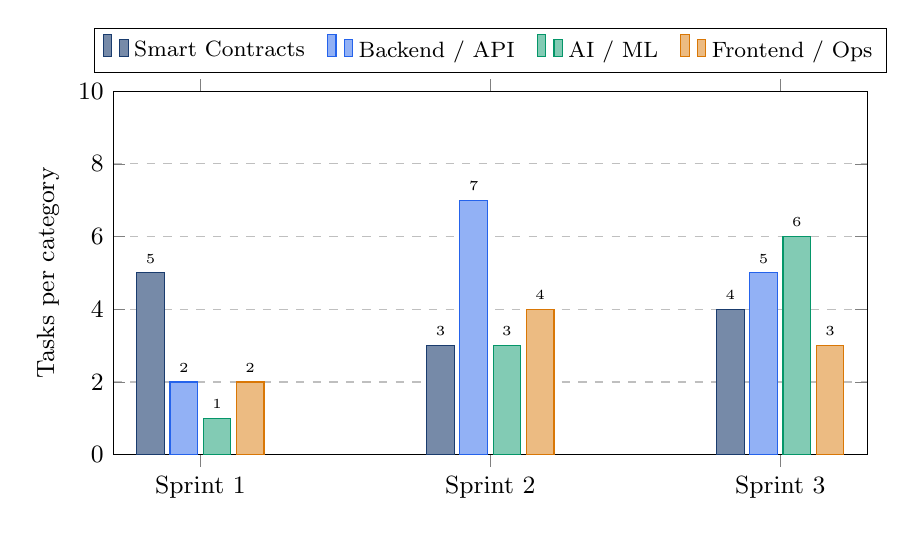
\begin{tikzpicture}
  \begin{axis}[
      ybar=2pt,
      bar width=10pt,
      width=0.92\linewidth, height=6.2cm,
      enlarge x limits=0.15,
      ymin=0, ymax=10,
      ylabel={Tasks per category},
      xtick=data,
      symbolic x coords={Sprint 1,Sprint 2,Sprint 3},
      ymajorgrids,
      grid style=dashed,
      tick label style={font=\small},
      label style={font=\small},
      legend style={font=\footnotesize, at={(0.5,1.05)}, anchor=south, legend columns=4, /tikz/every even column/.append style={column sep=0.6em}},
      nodes near coords,
      every node near coord/.append style={font=\tiny,/pgf/number format/.cd,fixed,precision=0},
  ]
    \addplot[draw=PrimaryBlue, fill=PrimaryBlue!60] coordinates {(Sprint 1,5) (Sprint 2,3) (Sprint 3,4)};
    \addplot[draw=AccentBlue, fill=AccentBlue!50] coordinates {(Sprint 1,2) (Sprint 2,7) (Sprint 3,5)};
    \addplot[draw=GreenAccent, fill=GreenAccent!50] coordinates {(Sprint 1,1) (Sprint 2,3) (Sprint 3,6)};
    \addplot[draw=AmberAccent, fill=AmberAccent!50] coordinates {(Sprint 1,2) (Sprint 2,4) (Sprint 3,3)};
    \legend{Smart Contracts, Backend / API, AI / ML, Frontend / Ops}
  \end{axis}
\end{tikzpicture}
\Description{Grouped bar chart showing task counts per sprint across four categories: Smart Contracts shows 5 in Sprint 1, 3 in Sprint 2, 4 in Sprint 3; Backend / API shows 2, 7, 5; AI / ML shows 1, 3, 6; Frontend / Ops shows 2, 4, 3.}
\caption{Sprint distribution by category. Sprint 1 is contracts-heavy (foundation), Sprint 2 expands the backend and frontend, Sprint 3 is AI / ML heavy and integration-heavy.}
\label{fig:sprint-dist}
\end{figure}

\section{Intelligent Services: Unified 9B Assistant}
\label{sec:ai-services}

The platform provides three intelligent services through a single 9-billion-parameter base model fine-tuned with QLoRA: a borrower-facing chatbot, an internal security advisory channel surfaced on pull requests, and a risk-explanation service that translates SHAP feature contributions into plain language. Figure~\ref{fig:ai-train} shows the training pipeline (data ingestion, JSONL builder, QLoRA training, merge, GGUF export). Figure~\ref{fig:ai-runtime} consolidates the runtime view with three panels: the assistant's inference flow with ChromaDB RAG, the production scoring pipeline with RF + IF + SHAP, and the CI security loop with Slither + Mythril + Echidna.

\CWBImprovedDiagram{fig-ai-training-pipeline}{AI training pipeline: data ingest, JSONL builder, QLoRA SFT, merge, GGUF export.}{Three-panel diagram. Panel A data pipeline: policy and thesis docs, SWC vulnerability pairs, synthetic loan dialogues, anonymised tx graphs feed SentenceTransformer embeddings to ChromaDB and a JSONL builder for SFT plus a tabular feature builder for RF, IF, SHAP. Panel B QLoRA training: base 9B 4-bit nf4 quant, LoRA adapters r=16 alpha=32, multi-task SFT chat security risk, merge weights, export GGUF Q4_K_M. Panel C deployment: llama.cpp server port 8080 and ChromaDB RAG feed FastAPI /v1/chat plus /risk-score.}{fig:ai-train}

\CWBImprovedDiagram{fig-ai-runtime-security}{Runtime view: unified 9B assistant, production scoring pipeline, CI security loop.}{Three-panel diagram. Panel A runtime unified 9B architecture: three inputs (borrower chat, security advisory, risk explanation) feed into RAG (security advisory branch) or tabular RF plus IF plus SHAP (risk branch), all converging on 9B QLoRA llama.cpp Q4_K_M, then output formatter plus safety filter. Panel B production scoring pipeline: on-chain tx plus session events through feature engineering to RF fraud probability and IF anomaly score, then composite 0.7 times RF plus 0.3 times IF, score band decision below 0.4 auto-approve, 0.4 to 0.7 manual review, 0.7 or above auto-reject plus SHAP. Panel C CI security loop: git push to Slither HIGH fails the PR, Mythril deep, Echidna fuzz, RAG index updated, 9B security advisory posted on PR.}{fig:ai-runtime}

\subsection{Base models and quantisation}
The base model is a 7--9B class general LLM (Llama-3-8B-Instruct or Mistral-7B-v0.3) quantised to 4-bit NF4. The reasoning is empirical: 7--9B class models are the smallest that can sustain coherent multi-turn dialogue while still fitting on a single consumer GPU after 4-bit quantisation (memory $\approx$ 6 GB). Export uses llama.cpp's GGUF Q4\_K\_M format, which preserves $\sim$95\% of full-precision accuracy on dialogue tasks at $\sim$4x throughput.

\subsection{Task specification and guardrails}
The assistant is trained on three task heads bundled into one model: (a)~borrower dialogue (FAQs, repayment status, limit checks), (b)~SWC vulnerability advisory (paired with vulnerable / patched Solidity snippets), and (c)~SHAP narrative generation (feature contributions to plain English). Guardrails are: no investment advice; no automatic financial-decision execution; PII redaction in logs; constrained decoding for value-bound outputs (numeric limits, percentages).

\subsection{Training data and QLoRA pipeline}
Training data comes from four sources: (i)~the policy and thesis corpus (this document, the BlockchainOlympiad guideline, World Bank publications); (ii)~SWC vulnerability--patch pairs scraped from public audit reports; (iii)~synthetic loan dialogues generated by GPT-4-class teacher models and then human-filtered; (iv)~anonymised transaction graphs from Polygon testnet. The QLoRA configuration is LoRA $r=16$, $\alpha=32$, learning rate $2 \times 10^{-4}$, batch size 8, 3 epochs, warmup 5\%.

\subsection{Evaluation}
\label{sec:llm-eval}
The LLM is evaluated on three axes:
\begin{enumerate}[leftmargin=*,itemsep=2pt]
    \item \textbf{Task accuracy:} F1 on a held-out 1k-example test set across the three task heads (target $\geq 0.85$).
    \item \textbf{Safety:} a held-out red-team set covering injection, jailbreak, hallucination, and financial-advice prompts. The adversarial-vulnerability paper~\cite{llmFinanceVuln2025} provides the threat catalogue. Target $\geq 0.95$ refusal accuracy on the red-team set.
    \item \textbf{Calibration:} the SHAP narrative head is evaluated against a held-out set of borrower-graded explanations (clarity, accuracy) with the protocol of Bracke et al.~\cite{bracke2019mlfinance}.
\end{enumerate}

\section{Federated Learning for Multi-Bank Fraud Intelligence}
\label{sec:fl}

The federated learning specification follows the PrivChain-AI~\cite{privchainAi2025} and Abbassi et al.~\cite{abbassi2025federated} designs: each Local Bank trains a local Random Forest + Isolation Forest model on its own data, and only the parameter deltas (not raw data) are sent to its parent National Bank, which aggregates via FedAvg (formula F.20). The aggregated regional model is then distributed back to all Local Banks. Cross-region aggregation at Tier 1 produces a global baseline. Figure~\ref{fig:fl} shows the topology.

\CWBImprovedDiagram{fig-federated-learning}{Federated learning topology: local training at Local Banks, FedAvg aggregation at National Banks, cross-region aggregation at the World Bank.}{Three-layer topology. Bottom layer Tier 3 Local Banks: LocalBank A, B, C each train local fraud model on private data. Middle layer Tier 2 National Bank: FedAvg aggregator weights only no raw data, then updated regional model. Top layer Tier 1 World Bank: cross-region FedAvg across National Banks, then global fraud baseline. Local banks send weight delta to aggregator, aggregator distributes regional weights back. Global baseline updates regional model.}{fig:fl}

\section{Graph Neural Network Extension}
\label{sec:gnn}

The Random Forest channel scores wallets independently. The 2024 GNN-on-DeFi-fraud literature~\cite{cheng2024gnnFraud,wang2024defiguard,wang2025gnnFraud} demonstrates that wallet-graph neighbourhood signals (e.g., k-hop transaction structure) materially improve fraud detection. The pre-thesis 2 deliverable adds a graph layer: the wallet graph for each Local Bank is built from on-chain events indexed by The Graph subgraph; a GraphSAGE model computes per-wallet embeddings; the embedding becomes a feature consumed by the existing RandomForest. Ablation against the current tabular-only RF will be the empirical validation.

\section{Formal Verification with Certora}
\label{sec:certora}

Following the Certora 2025 open-source release~\cite{certoraOpenSource2025}, two CVL invariants are specified on the reserve contract:

\begin{enumerate}[leftmargin=*,itemsep=2pt]
    \item \textbf{Reserve solvency.} \texttt{totalAllocated <= reserveBalance + sum(returnedSurplus)}: the WorldBankReserve never allocates more than it has received.
    \item \textbf{Role segregation.} No address can simultaneously hold both \texttt{LOAN\_APPROVER\_ROLE} and \texttt{BORROWER\_ROLE} for the same loan.
\end{enumerate}

These two properties cover the two highest-impact failure modes (insolvency at Tier 1 and approver self-dealing). Certora's CVL specification is sketched in Appendix~\ref{app:certora}; the proof is part of pre-thesis 2.

\section{Foundry Invariant and Fuzz Test Suite}
\label{sec:foundry}

The current scaffold has Hardhat unit tests only. Pre-thesis 2 introduces a Foundry invariant + fuzz suite covering:

\begin{itemize}[leftmargin=*,itemsep=2pt]
    \item \textbf{Solvency invariant.} For every reachable state, sum of LocalBank balances $\leq$ sum allocated by NationalBanks.
    \item \textbf{Role-expiry invariant.} No expired role is honoured by any guarded function.
    \item \textbf{Rolling-limit fuzz.} Over a fuzzed sequence of loan requests, the cumulative 180-day disbursement to any borrower $\leq$ the tier ceiling at every moment.
    \item \textbf{HF boundary fuzz.} On randomly sampled $(C, D, LT, \text{price})$ quadruples, the liquidation engine triggers iff F.7 evaluates below 1.0.
    \item \textbf{Pause boundary fuzz.} Each granular pause flag suppresses its target function and only its target function.
\end{itemize}

The Foundry suite is integrated in the CI pipeline (Figure~\ref{fig:test-pipeline}).

\CWBImprovedDiagram{fig-test-pipeline}{CI test pipeline: Hardhat unit + integration, Foundry fuzz + invariant, Slither static, Mythril deep, Echidna property, Halmos / Certora pre-demo.}{Horizontal flow. git push to GitHub Actions CI decision, then hardhat compile, hardhat unit plus integration, hardhat Polygon Amoy fork tests, Foundry forge test, Foundry fuzz borrowing limit boundaries, Foundry invariant solvency role segregation, Slither static analysis fail on HIGH, Mythril deep symbolic nightly, Echidna property fuzz weekly, Halmos and Certora pre-demo, decision coverage greater than or equal to 80 percent, if no fail PR if yes deploy preview to Amoy.}{fig:test-pipeline}

\section{Agent-Based Economic Feasibility Simulation}
\label{sec:abm}

A discrete-event agent-based simulation will validate the unit economics claimed in Chapter~\ref{ch:market}. Each agent class -- World Bank, National Banks, Local Banks, retail borrowers, group borrowers, liquidators -- has a behavioural rule. The simulation runs over 36 simulated months sweeping default rate (5\%--15\%) and average loan size (USD 100--1000); the output is per-tier annualised return, default-induced capital depletion, and liquidation throughput. The simulation is implemented in Mesa (Python) for pre-thesis 2.

\section{Real-Time Dashboard Pipeline}
\label{sec:dashboard}

Real-time visibility is critical for institutional confidence. The pipeline (Figure~\ref{fig:dashboard}) ingests on-chain events via an ethers WebSocketProvider, persists them in PostgreSQL, publishes through a Redis pub/sub channel, and pushes to React clients over Socket.io. Historical queries fall back to PostgreSQL; portfolio summaries fall back to The Graph.

\CWBImprovedDiagram{fig-realtime-dashboard}{Real-time dashboard pipeline.}{Architecture flow. Polygon Amoy contract events via ethers WebSocketProvider to Express event listener. Listener ingests to PostgreSQL and Redis pub/sub. Redis subscribers feed Socket.io server, which emits to React client room loan-id. Client renders toast or update card. Historical queries from PostgreSQL and GraphQL queries from The Graph subgraph go to the client.}{fig:dashboard}

\section{Transaction State Machine}
\label{sec:tx-state}

Every borrower-initiated transaction (loan request, repayment, vault deposit) follows the state machine of Figure~\ref{fig:tx-state}. Replaced transactions (gas-price-bumped by the wallet) are tracked through the new hash so the UI does not show false errors. Reverted transactions are surfaced with the decoded revert reason. This is part of the accessibility-design considerations of Section~\ref{sec:accessibility}.

\CWBImprovedDiagram{fig-tx-state-machine}{Transaction lifecycle state machine.}{State diagram. Initial IDLE. Transitions: IDLE to PENDING SIGNATURE on user clicks Pay; PENDING SIGNATURE to SUBMITTED on wallet signs or to ERROR on user rejects; SUBMITTED to CONFIRMING on broadcast ok or to ERROR on rpc failure; CONFIRMING to SUCCESS on greater than or equal to 1 confirmation, to REPLACED on tx replaced or sped up, or to ERROR on reverted; REPLACED to CONFIRMING on new hash tracked; SUCCESS to terminal; ERROR to IDLE on retry. Note UI shows progress bar with explorer link.}{fig:tx-state}

\section{EIP-712 Authentication Sequence}
\label{sec:eip712}
Wallet-signed JWT replaces password authentication. Figure~\ref{fig:eip712} shows the full challenge--sign--verify--JWT--blacklist flow. The JWT access token expires in 15 minutes; the refresh token expires in 7 days; logout blacklists the \texttt{jti} in Redis until natural expiry.

\CWBImprovedDiagram{fig-eip712-auth}{EIP-712 wallet-signed authentication: challenge, signature verification, JWT issuance, and Redis blacklist on logout.}{Sequence diagram with User, React dApp, Wallet AA or EOA, Express API, Redis. Steps: connect wallet, GET auth challenge with address, build EIP-712 challenge with domain nonce timestamp, returned challenge JSON, signTypedData v4 of challenge, returned signature, POST auth verify with addr and sig, ecrecover plus verify, SET session jti 15 min in Redis, returned JWT access 15 min plus refresh 7 days. All write endpoints require Authorization Bearer. POST loans with Bearer JWT, EXISTS blacklist jti, not blacklisted, 200 OK. Note logout blacklists jti until token natural expiry.}{fig:eip712}

\section{Evaluation Methodology}
\label{sec:eval-method}

Evaluation is split into smart-contract validation, ML validation, and end-to-end integration validation. Table~\ref{tab:eval-targets} fixes the quantitative targets.

\begin{table}[!t]
\centering
\caption{Quantitative evaluation targets for the final thesis.}
\label{tab:eval-targets}
\small
\begin{tabularx}{\linewidth}{@{}p{4.0cm}YR{2.8cm}@{}}
\toprule
\textbf{Metric} & \textbf{Component} & \textbf{Target} \\
\midrule
Line + branch coverage & Smart contracts (Hardhat + Foundry) & $\geq 80\%$ \\
Slither HIGH findings & Smart contracts & 0 \\
Mythril critical findings & Smart contracts & 0 \\
Echidna invariant violations & Smart contracts & 0 \\
Certora CVL proofs (reserve) & Smart contracts & 2 proven \\
ROC-AUC on RF fraud classifier & ML & $\geq 0.92$ \\
F1 on RF fraud classifier & ML & $\geq 0.85$ \\
Anomaly detection PR-AUC (IF) & ML & $\geq 0.85$ \\
9B assistant task F1 (3 heads avg) & LLM & $\geq 0.85$ \\
9B red-team refusal accuracy & LLM safety & $\geq 0.95$ \\
End-to-end loan latency (request $\to$ disbursed) & E2E & $\leq 15\,\mathrm{s}$ \\
WebSocket round-trip latency (dashboard) & E2E & $\leq 250\,\mathrm{ms}$ \\
\bottomrule
\end{tabularx}
\end{table}

\section{Sprint Plan and Deliverables}
\label{sec:sprint}

\begin{table}[!t]
\centering
\caption{Sprint 1 backlog (architecture and contracts foundation).}
\label{tab:sprint-1}
\small
\begin{tabularx}{\linewidth}{@{}lYR{1.6cm}@{}}
\toprule
\textbf{ID} & \textbf{Deliverable} & \textbf{Status} \\
\midrule
S1.1 & WorldBankReserve + allocation functions & \tmarkDone \\
S1.2 & NationalBank scaffold + registration & \tmarkPartial \\
S1.3 & LocalBank scaffold + disbursement & \tmarkPartial \\
S1.4 & Loan + Repayment data model + SQL migrations & \tmarkDone \\
S1.5 & PostgreSQL + Redis docker-compose & \tmarkDone \\
S1.6 & EIP-712 challenge endpoint + JWT issue/verify & \tmarkDone \\
S1.7 & React dApp shell + market data + AI chatbot stub & \tmarkPartial \\
S1.8 & Improved mermaid diagram set (43 figures) & \tmarkDone \\
S1.9 & Pre-thesis v14 LaTeX overhaul & \tmarkDone \\
\bottomrule
\end{tabularx}
\end{table}

\begin{table}[!t]
\centering
\caption{Sprint 2 backlog (AI/ML and governance specification).}
\label{tab:sprint-2}
\small
\begin{tabularx}{\linewidth}{@{}lYR{1.6cm}@{}}
\toprule
\textbf{ID} & \textbf{Deliverable} & \textbf{Status} \\
\midrule
S2.1 & FastAPI ML service: RF + IF + SHAP & \tmarkPartial \\
S2.2 & 9B QLoRA training data preparation & \tmarkPlanned \\
S2.3 & LiquidationEngine specification (this chapter) & \tmarkDone \\
S2.4 & SavingsVault + FixedDeposit specification & \tmarkDone \\
S2.5 & Borrower limit engine + Redis cache & \tmarkPartial \\
S2.6 & The Graph subgraph schema & \tmarkPlanned \\
S2.7 & Safe multisig + TimeLock deployment script & \tmarkPlanned \\
S2.8 & MiCA + GENIUS Act compliance mapping & \tmarkDone \\
S2.9 & Foundry test scaffold + 5 invariants & \tmarkPlanned \\
S2.10 & ChromaDB RAG ingestion of policy corpus & \tmarkPlanned \\
\bottomrule
\end{tabularx}
\end{table}

\begin{table}[!t]
\centering
\caption{Sprint 3 backlog (integration + verification for pre-thesis 2).}
\label{tab:sprint-3}
\small
\begin{tabularx}{\linewidth}{@{}lYR{1.6cm}@{}}
\toprule
\textbf{ID} & \textbf{Deliverable} & \textbf{Status} \\
\midrule
S3.1 & Commit--reveal oracle wiring (LoanController) & \tmarkPlanned \\
S3.2 & Chainlink Functions migration & \tmarkPlanned \\
S3.3 & KYCVerifier Circom 2.0 circuit + integration & \tmarkPlanned \\
S3.4 & AMLVerifier zkAML circuit + Merkle root refresh & \tmarkPlanned \\
S3.5 & CreditPassportSBT (ERC-5114-like) & \tmarkPlanned \\
S3.6 & Federated FedAvg aggregator (Tier 2) & \tmarkPlanned \\
S3.7 & GraphSAGE ablation against tabular RF & \tmarkPlanned \\
S3.8 & Certora CVL proofs (reserve solvency, role segregation) & \tmarkPlanned \\
S3.9 & Tenderly monitor + 6 alert triggers configured & \tmarkPlanned \\
S3.10 & Bridge candidate evaluation (LayerZero / Axelar / CCIP) & \tmarkPlanned \\
S3.11 & Mesa agent-based feasibility simulation & \tmarkPlanned \\
S3.12 & End-to-end demo on Polygon Amoy & \tmarkPlanned \\
\bottomrule
\end{tabularx}
\end{table}

\section{SDLC Stage Mapping}
\label{sec:sdlc}

Pre-thesis 1 covers the requirements, design, partial implementation, and unit-test phases of the classical SDLC. Pre-thesis 2 covers integration, system testing, formal verification, and acceptance. The agile sprint structure is overlaid on this classical phase decomposition (Table~\ref{tab:sdlc}).

\begin{table}[!t]
\centering
\caption{SDLC stage mapping.}
\label{tab:sdlc}
\small
\begin{tabularx}{\linewidth}{@{}llY@{}}
\toprule
\textbf{Phase} & \textbf{Sprint} & \textbf{Output} \\
\midrule
Requirements & S1 & Stakeholder analysis, use cases, BB SP2025-02 grounding \\
Design & S1, S2 & Architecture (Ch. 3), 43 improved diagrams \\
Implementation (partial) & S1, S2 & Reserve, NB, LB scaffolds; FastAPI ML; React dApp \\
Unit testing & S2 & Hardhat unit tests, Pytest ML tests \\
Integration testing & S3 & Hardhat fork tests + Foundry invariants \\
Formal verification & S3 & Certora CVL proofs \\
System / acceptance testing & S3 & End-to-end demo, agent simulation \\
\bottomrule
\end{tabularx}
\end{table}

\section{Design Decisions and Alternatives}
\label{sec:design-decisions}

The principal design decisions and their alternatives are catalogued in Table~\ref{tab:design-decisions}. Each row pairs an alternative with the reason the chosen path was preferred.

\begin{table}[!t]
\centering
\caption{Design decisions and alternatives.}
\label{tab:design-decisions}
\small
\begin{tabularx}{\linewidth}{@{}p{3.6cm}p{3.4cm}Y@{}}
\toprule
\textbf{Decision} & \textbf{Chosen vs. alternative} & \textbf{Rationale} \\
\midrule
L1 chain & Polygon Amoy vs.\ Ethereum mainnet & USD 0.01--0.05 gas per op vs.\ USD 5--15; PoS finality $\sim$5s; mainnet deferred \\
Loan denomination & Stablecoin vs.\ native ETH & MiCA + GENIUS; eliminates volatility doubling real debt in drawdown \\
Identity layer & DID + VC + ZKP vs.\ raw on-chain PII & SSI; GDPR / PDPA compliance; on-chain stores flag only \\
Upgrade pattern & UUPS vs.\ Transparent Proxy vs.\ Beacon & Cheaper proxy calls; upgrade logic in implementation; auditable via TimeLock \\
Multisig & Safe 3-of-5 vs.\ single EOA & Single-key compromise unacceptable; 3-of-5 supports staff rotation \\
Risk pipeline & Commit-reveal oracle vs.\ direct on-chain ML & On-chain ML infeasible; commit-reveal prevents relay manipulation \\
ML model & RF + IF + SHAP vs.\ pure neural & SHAP-friendly; interpretable; small training set sufficient \\
LLM & 9B QLoRA vs.\ API call to GPT-4 & Cost predictability; on-prem privacy; deterministic version \\
KYC provider & Veriff vs.\ Persona vs.\ Sumsub & Bangladesh coverage; sandbox-compatible API; price competitive \\
SBT standard & ERC-5114-like vs.\ ERC-721 transferable & Non-transferable is the point; resists capture and sale \\
Bridge & Defer decision to pre-thesis 2 & 2022--2024 bridge hacks history; need empirical evaluation \\
Liquidation incentive & 5--8\% keeper bonus vs.\ DAO fund & Permissionless keeping; aligns with Aave V3 norms \\
\bottomrule
\end{tabularx}
\end{table}

\section{Design Patterns}
\label{sec:patterns}

\begin{table}[!t]
\centering
\caption{Software design patterns applied.}
\label{tab:patterns}
\small
\begin{tabularx}{\linewidth}{@{}lYY@{}}
\toprule
\textbf{Pattern} & \textbf{Application in CWB} & \textbf{Layer} \\
\midrule
Proxy (UUPS) & WorldBankReserve, LB, NB upgradeable & L1 contract \\
Factory & LocalBankContract deployed per Local Bank & L1 contract \\
Observer & The Graph subgraph subscribes to events & L4 indexing \\
State Machine & Loan lifecycle (Figure~\ref{fig:tx-state}) & L1 + L7 \\
Strategy & RF + IF composite scoring & L3 ML \\
Adapter & CWBPriceFeed wraps Chainlink + CoinGecko & L1 contract \\
Repository & DAOs over PostgreSQL in Express & L2 application \\
Singleton & WorldBankReserve (single global) & L1 contract \\
Circuit Breaker & Granular pause states (Figure~\ref{fig:pause}) & L1 contract \\
Saga & Cross-tier allocation with compensating reverts & L1 + L2 \\
\bottomrule
\end{tabularx}
\end{table}

\section{Software Testing Strategy}
\label{sec:testing-strategy}

The testing strategy combines unit tests (Hardhat for contracts, Pytest for ML), property tests (Foundry invariants + fuzz), static analysis (Slither, Mythril, Echidna), formal verification (Certora CVL), integration tests on Polygon Amoy fork, and an end-to-end demo. The pipeline structure is Figure~\ref{fig:test-pipeline}; coverage targets are in Table~\ref{tab:eval-targets}.

%% %%%%%%%%%%%%%%%%%%%%%%%%%%%%%%%%%%%%%%%%%%%%%%%%%%%%%%%%%%%%
%% CHAPTER 5: MARKET ANALYSIS AND FEASIBILITY
%% %%%%%%%%%%%%%%%%%%%%%%%%%%%%%%%%%%%%%%%%%%%%%%%%%%%%%%%%%%%%
\chapter{Market Analysis and Feasibility}
\label{ch:market}

\section{Market Sizing}
\label{sec:market-sizing}

The funnel of Figure~\ref{fig:market-opportunity} resolves to: \textbf{TAM} (Total Addressable Market) of USD 18 trillion across global SME finance, remittances, and microcredit; \textbf{SAM} (Serviceable Addressable Market) of USD 850 billion across emerging-market mobile-first credit; \textbf{SOM} (Serviceable Obtainable Market) of USD 14 billion across Bangladesh + South Asia digital-lender share over five years. The Bangladesh-specific anchor is the 41.56 million microfinance accounts reported by Bangladesh Bank~\cite{bangladeshBank2025} and the women-led BRAC microfinance reach reported in 2025~\cite{brac2025microfinance}.

\section{Target Customer Segment}
\label{sec:customer}

The primary customer segment is women-led solidarity-group microbusinesses in Bangladesh's rural and peri-urban districts (10--12 borrower groups around each Local Bank operator). The secondary segment is SMEs that fall through MFI ceilings but below commercial-bank floors -- the USD 3,000--30,000 monthly turnover band -- with documented MSME credit gap of USD 5.2 trillion globally~\cite{ifc2019msme} and Bangladesh share approximately USD 150 billion. The tertiary segment is institutional allocators (development banks, donor agencies) channeling capital through Local Banks.

\section{Partner Ecosystem}
\label{sec:partner}

Five partner classes are required to reach the customer segments above: (i)~\textit{Local Bank operators} (BRAC Bank pilot, Eastern Bank pilot, ASA digital pilot); (ii)~\textit{KYC providers} (Veriff, Persona, Sumsub) -- evaluated on Bangladesh NID coverage; (iii)~\textit{stablecoin issuers / on-ramps} (Circle USDC, Tether USDT, Stellar XLM USDC pair via Stellar Disbursement Platform~\cite{stellar2025report}); (iv)~\textit{infrastructure} (Polygon Foundation, Chainlink, Alchemy / Biconomy for AA, Tenderly, OpenZeppelin Defender); (v)~\textit{academic / NGO partners} (BRAC Microfinance, BRAC Institute of Governance and Development, Grameen Foundation).

\section{Phased Go-to-Market}
\label{sec:gtm}
Figure~\ref{fig:gtm} situates CWB in the institutional-blockchain adoption timeline (JPM Onyx 2020, Aave V3 multi-chain 2022, BIS mBridge MVP 2024, MiCA full effect 2026, CWB pilot target 2027) and decomposes the deployment into four phases: validation (BRAC University pilot, 20 retail wallets), sandbox (Bangladesh Bank RFFO, USD 50K loans), production (three Local Banks, USD 2M ARR), and regional scale (South Asia, USD 20M ARR).

\CWBImprovedDiagram{fig-go-to-market}{Institutional-blockchain adoption timeline and CWB phased go-to-market.}{Two-panel diagram. Panel A timeline 2020 JPM Onyx, 2022 Aave V3 multi-chain, 2024 BIS mBridge MVP, 2025 GENIUS Act and Certora OSS, 2026 MiCA full effect, 2027 CWB pilot target. Panel B four GTM phases: Phase 1 M0-M6 Validation BRAC pilot 20 retail wallets; Phase 2 M6-M12 Sandbox pilot BB RFFO USD 50K loans; Phase 3 M12-M24 Production three Local Banks USD 2M ARR; Phase 4 M24+ Regional scale South Asia USD 20M ARR.}{fig:gtm}

\section{Competitive Landscape}
\label{sec:competitive}

Figure~\ref{fig:competitive} shows the four-quadrant positioning of CWB against eleven competitors. The unique position is the top-right (institutional + multi-tier) quadrant.

\CWBImprovedDiagram{fig-competitive-landscape}{Quadrant chart of competitors. The CWB position is institutional + multi-tier (top right).}{Quadrant chart with X axis retail-only to institutional plus retail and Y axis flat pool architecture to hierarchical or multi-tier. Quadrant 1 is multi-tier institutional CWB whitespace. Quadrant 2 is tiered MFI / TradFi. Quadrant 3 is retail-only flat DeFi. Quadrant 4 is institutional flat DeFi. Points: Aave 0.30, 0.20; Compound 0.25, 0.18; Morpho 0.45, 0.30; Maple 0.75, 0.32; Goldfinch 0.55, 0.42; MakerDAO 0.40, 0.25; Grameen 0.20, 0.78; BRAC Microfinance 0.22, 0.80; JPM Onyx 0.85, 0.65; BIS mBridge 0.95, 0.55; Crypto World Bank 0.78, 0.88.}{fig:competitive}

Table~\ref{tab:competitor-detail} consolidates the three separate competitor tables of v13 (Direct DeFi, TradFi institutional, regional Asia/microfinance) into a single wide booktabs table with thirteen rows.

\begin{table}[!t]
\centering
\caption{Consolidated competitive landscape (DeFi, TradFi institutional, regional / microfinance).}
\label{tab:competitor-detail}
\small
\setlength{\tabcolsep}{4pt}
\begin{tabularx}{\linewidth}{@{}p{2.4cm}p{1.6cm}p{1.8cm}YY@{}}
\toprule
\textbf{Competitor} & \textbf{Class} & \textbf{TVL or AUM (2026)} & \textbf{Strength} & \textbf{Gap} \\
\midrule
Aave V3~\cite{defillamaAaveV3} & DeFi & USD 25B & Composability, mature & Flat pool; no hierarchy \\
Compound V3~\cite{defillamaCompoundV3} & DeFi & USD 4B & Audited, stable & Flat pool; no hierarchy \\
Morpho~\cite{morphoData} & DeFi & USD 12B & Vault customisation & No institutional governance \\
Sky / MakerDAO~\cite{fensorySky2026} & DeFi & USD 20.6B & Stablecoin issuance & Single-tier \\
Maple Finance~\cite{fensoryMaple2026} & DeFi (institutional) & USD 2B & Institutional pools & No retail tier \\
Goldfinch & DeFi (RWA) & USD 200M & RWA collateral & No hierarchical reserve \\
Centrifuge~\cite{centrifugeRwa2025} & DeFi (RWA) & USD 700M & RWA tokenisation & No retail tier \\
JPM Onyx (Kinexys)~\cite{jpmKinexys2025} & TradFi & USD 1.5T settled & Institutional grade & Closed network \\
BIS mBridge~\cite{bisMbridge2024} & TradFi & MVP & Sovereign CBDC bridge & Settlement only; no lending \\
Project Agora~\cite{bisAgora2024} & TradFi & Pilot & Unified ledger & Settlement only \\
Grameen Bank & MFI & USD 1.2B & Solidarity model proven & Off-chain; no portability \\
BRAC Microfinance~\cite{brac2025microfinance} & MFI & USD 4B & Reach + women focus & Off-chain; no portability \\
\textbf{Crypto World Bank} & DeFi + MFI hybrid & --- & Multi-tier + AI + ZKP + SBT & Pilot scale (this work) \\
\bottomrule
\end{tabularx}
\end{table}

\section{Risk Taxonomy}
\label{sec:risk-taxonomy}

Table~\ref{tab:risks} consolidates technical, market, and regulatory risks with mitigation.

\begin{table}[!t]
\centering
\caption{Risk taxonomy with mitigation.}
\label{tab:risks}
\small
\begin{tabularx}{\linewidth}{@{}p{2.3cm}YY@{}}
\toprule
\textbf{Risk class} & \textbf{Specific risk} & \textbf{Mitigation} \\
\midrule
Technical & Smart contract bug & 4-tool audit pipeline + Certora CVL proofs \\
Technical & Oracle manipulation & Commit-reveal + Chainlink Price Feed + staleness check \\
Technical & Bridge hack & Single-chain pre-MVP; bridge evaluation in pre-thesis 2 \\
Market & Stablecoin de-peg~\cite{stablecoinDevaluation2025} & Diversify across USDC + USDT + planned local-CBDC \\
Market & Borrower default cluster & Solidarity-group joint liability + 5--8\% liquidation bonus \\
Market & Over-indebtedness (cross-platform)~\cite{nusMicrofinance2025} & CreditPassportSBT + cap on simultaneous active loans \\
Regulatory & MiCA non-compliance & 1:1 reserve + authorisation + audit (Section~\ref{sec:stablecoin}) \\
Regulatory & GENIUS Act non-compliance & USDC integration + licensed issuer custody \\
Regulatory & Bangladesh sandbox rejection & Pilot scope aligned with FE Circular No.~06 + RFFO sandbox \\
Operational & Safe signer compromise & 3-of-5 multisig + hardware + key rotation policy \\
Operational & ML data drift & Quarterly re-training + Tenderly drift alerts \\
\bottomrule
\end{tabularx}
\end{table}

\section{Technical Feasibility}
\label{sec:tech-feasibility}

Per-loan gas cost on Polygon Amoy is dominated by storage writes: loan creation $\approx$ 230k gas, repayment $\approx$ 95k gas, liquidation $\approx$ 320k gas. At Polygon's gas-token price ($\sim$0.05 GWEI MATIC, $\sim$USD 0.50/MATIC), one full loan lifecycle costs less than USD 0.05 -- two orders of magnitude below the spread captured by the platform. ML inference per scoring call is $\sim$120 ms on a single CPU core with the FastAPI service; the QLoRA assistant returns first token within 1.2 s on consumer-grade GPU.

\section{Economic Feasibility}
\label{sec:econ-feasibility}

Net interest allocation (formula F.16) under the kinked rate model (Section~\ref{sec:kinked}) for a representative Local Bank with USD 100k portfolio at 65\% utilisation yields a $\sim$2\% net spread after depositor yield and 0.5\% insurance allocation. Per the agent-based simulation (Section~\ref{sec:abm}) at 8\% default rate, capital recovery from the LiquidationEngine + insurance pool keeps Local Bank capital depletion below 1.5\% per annum -- below the spread.

\section{Revenue Projection}
\label{sec:revenue}

Figure~\ref{fig:revenue-tier} (refurbished from v13) shows the projected annual revenue by tier under steady-state operating assumptions of the agent-based simulation; Figure~\ref{fig:rate-spread} (refurbished from v13) shows the hierarchical interest-rate spread; Figure~\ref{fig:revenue-sens} (new in v14) shows the revenue sensitivity to default rate and average loan size.

\begin{figure}[!t]
\centering
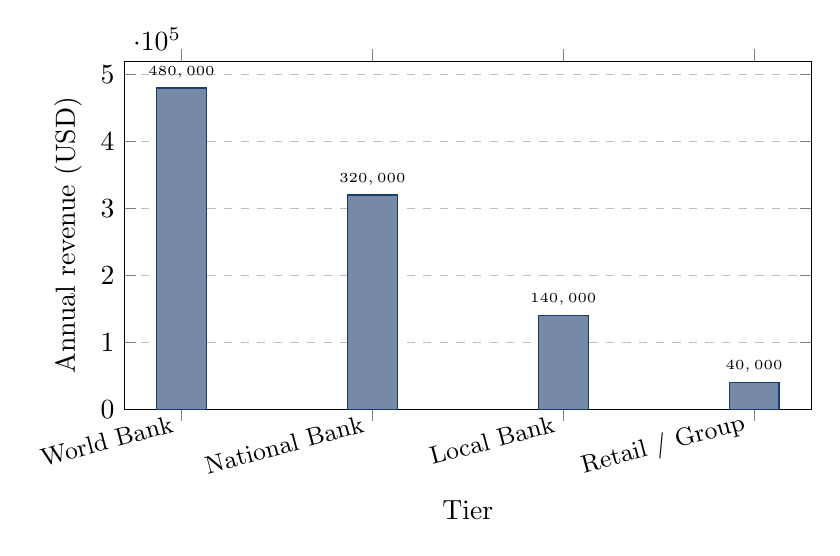
\begin{tikzpicture}
  \begin{axis}[
      ybar,
      bar width=18pt,
      width=0.85\linewidth, height=6cm,
      ymin=0, ymax=520000,
      ylabel={Annual revenue (USD)},
      xlabel={Tier},
      symbolic x coords={World Bank, National Bank, Local Bank, Retail / Group},
      xtick=data,
      x tick label style={font=\small, rotate=15, anchor=east},
      nodes near coords,
      every node near coord/.append style={font=\tiny, /pgf/number format/.cd, fixed, 1000 sep={,}},
      ymajorgrids,
      grid style=dashed,
      ytick={0,100000,200000,300000,400000,500000},
      yticklabel={\pgfmathprintnumber[fixed, 1000 sep={,}]{\tick}},
  ]
    \addplot[draw=PrimaryBlue, fill=PrimaryBlue!60] coordinates {(World Bank,480000) (National Bank,320000) (Local Bank,140000) (Retail / Group,40000)};
  \end{axis}
\end{tikzpicture}
\Description{Bar chart of projected annual revenue by tier. World Bank approximately 480000 dollars, National Bank approximately 320000 dollars, Local Bank approximately 140000 dollars, Retail / Group approximately 40000 dollars.}
\caption{Projected annual revenue by tier under the agent-based simulation steady state. Year-3 production scale, three Local Banks, USD 2M aggregate ARR.}
\label{fig:revenue-tier}
\end{figure}

\begin{figure}[!t]
\centering
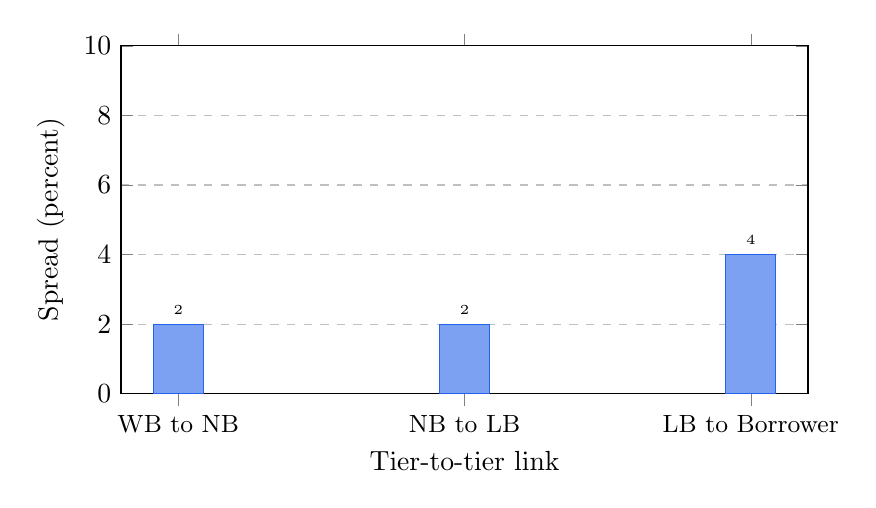
\begin{tikzpicture}
  \begin{axis}[
      ybar,
      bar width=18pt,
      width=0.85\linewidth, height=6cm,
      ymin=0, ymax=10,
      ylabel={Spread (percent)},
      xlabel={Tier-to-tier link},
      symbolic x coords={WB to NB, NB to LB, LB to Borrower},
      xtick=data,
      x tick label style={font=\small},
      nodes near coords,
      every node near coord/.append style={font=\tiny},
      ymajorgrids,
      grid style=dashed,
  ]
    \addplot[draw=AccentBlue, fill=AccentBlue!60] coordinates {(WB to NB,2) (NB to LB,2) (LB to Borrower,4)};
  \end{axis}
\end{tikzpicture}
\Description{Bar chart of interest-rate spread across the hierarchy. WB to NB spread approximately 2 percent, NB to LB spread approximately 2 percent, LB to Borrower spread approximately 4 percent.}
\caption{Hierarchical interest-rate spread: cumulative borrower APR of $\sim$8\% is consistent with the waterfall in Figure~\ref{fig:economic}.}
\label{fig:rate-spread}
\end{figure}

\begin{figure}[!t]
\centering
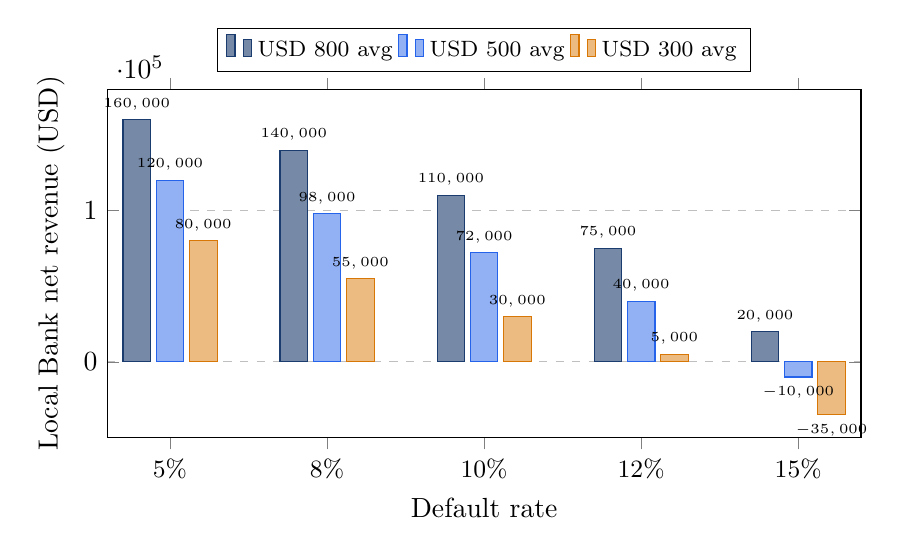
\begin{tikzpicture}
  \begin{axis}[
      ybar=2pt,
      bar width=10pt,
      width=0.92\linewidth, height=6cm,
      ymin=-50000, ymax=180000,
      ylabel={Local Bank net revenue (USD)},
      xlabel={Default rate},
      symbolic x coords={5\%, 8\%, 10\%, 12\%, 15\%},
      xtick=data,
      x tick label style={font=\small},
      ymajorgrids,
      grid style=dashed,
      yticklabel={\pgfmathprintnumber[fixed, 1000 sep={,}]{\tick}},
      legend style={font=\footnotesize, at={(0.5,1.05)}, anchor=south, legend columns=3},
      nodes near coords,
      every node near coord/.append style={font=\tiny, /pgf/number format/.cd, fixed, 1000 sep={,}},
  ]
    \addplot[draw=PrimaryBlue, fill=PrimaryBlue!60] coordinates {(5\%,160000) (8\%,140000) (10\%,110000) (12\%,75000) (15\%,20000)};
    \addplot[draw=AccentBlue, fill=AccentBlue!50] coordinates {(5\%,120000) (8\%,98000) (10\%,72000) (12\%,40000) (15\%,-10000)};
    \addplot[draw=AmberAccent, fill=AmberAccent!50] coordinates {(5\%,80000) (8\%,55000) (10\%,30000) (12\%,5000) (15\%,-35000)};
    \legend{USD 800 avg, USD 500 avg, USD 300 avg}
  \end{axis}
\end{tikzpicture}
\Description{Grouped bar chart of revenue sensitivity. X-axis shows default rate 5, 8, 10, 12, 15 percent. Y-axis shows net revenue dropping from approximately 160000 to 20000 dollars at USD 800 average loan, from 120000 to negative 10000 dollars at USD 500 average loan, and from 80000 to negative 35000 dollars at USD 300 average loan.}
\caption{Revenue sensitivity to default rate and average loan size for a representative Local Bank. The USD 300 average loan turns unprofitable above 12\% default; the over-indebtedness controls of Section~\ref{sec:over-indebt} keep portfolio default below this band.}
\label{fig:revenue-sens}
\end{figure}

\section{Currency Risk and Stablecoin Imperative}
\label{sec:currency}
The volatile-collateral analysis of v13 is extended in v14 with the explicit MiCA + GENIUS compliance mapping (Section~\ref{sec:stablecoin} and Appendix~\ref{app:compliance}). The empirical justification for the stablecoin-first design is the May 2021 and 2022 ETH drawdowns of 50\% within months, doubling real borrower debt where loans were denominated in ETH.

\section{Bootstrap Funding and Tier 1 Capitalization}
\label{sec:bootstrap}

\begin{table}[!t]
\centering
\caption{Funding sources for Tier 1 capitalization.}
\label{tab:funding}
\small
\begin{tabularx}{\linewidth}{@{}p{3.6cm}p{2.6cm}Y@{}}
\toprule
\textbf{Source} & \textbf{Stage} & \textbf{Notes} \\
\midrule
University seed grant & Pilot & BRAC University CSE seed pool (in-kind) \\
Polygon Foundation grant & Pilot & Polygon Village programme for civic apps \\
DAO treasury (Aave Grants DAO) & Sandbox & Aave grants for Aave-V3-compatible protocols \\
Stellar Community Fund~\cite{stellar2025report} & Sandbox & Microfinance focus + Stellar Disbursement \\
World Bank Innovation Hub & Production & Project-level grant through MDB programmes \\
Donor cohort (BMGF, USAID) & Production & Microfinance digitisation focus area \\
National Bank pilot equity & Production & Local Bank operator co-investment \\
\bottomrule
\end{tabularx}
\end{table}

\section{Over-Indebtedness Risk in Group Lending}
\label{sec:over-indebt}

The NUS 2025 microfinance analysis~\cite{nusMicrofinance2025} documents that with 724 licensed MFIs in Bangladesh serving 41.56 million accounts, individual borrowers frequently service simultaneous loans from multiple institutions -- a structural over-indebtedness risk that solidarity-group guarantees alone do not solve. CWB's two mitigation controls are (a)~the CreditPassportSBT exposing cumulative active debt across compatible lenders (Section~\ref{sec:sbt}), allowing any querying lender to refuse a loan that would push total debt beyond a sustainable threshold; and (b)~a hard on-chain cap on the number of simultaneously active loans per borrower (default 2; configurable per Local Bank). Both controls are unenforceable in the current paper-based MFI ecosystem and are the principal social-impact contribution of the architecture.

\section{Prototype Scope and Limitations}
\label{sec:proto-limits}

The pre-thesis 1 deliverable is bounded by: (a)~Polygon Amoy testnet only, no mainnet; (b)~test stablecoins, no production stablecoin custody; (c)~mock KYC documents, no production KYC provider integration; (d)~the BRAC University pilot cohort only, no public users; (e)~simulated AI risk scores, full ML pipeline integration in pre-thesis 2.

\section{Accessibility Design Considerations}
\label{sec:accessibility}

Every figure in v14 carries a \texttt{\textbackslash Description\{\}} alt-text body (the requirement on the macro is enforced in Section~\ref{sec:high-arch}). Tables are designed with sufficient horizontal whitespace and no decorative row shading per ACM convention. The React dApp inherits Tailwind's accessibility tokens (focus rings, semantic colour, ARIA roles). The transaction state machine (Figure~\ref{fig:tx-state}) is a deliberate accessibility design choice: a clear UI for ``pending'', ``confirming'', ``success'', ``replaced'', ``error'' states reduces cognitive load for first-time crypto users.

\section{Statement of Contributions}
\label{sec:contributions}

\textbf{Pre-thesis 1.} M.B.R.J.\ and M.M.A.A.\ jointly developed the four-tier architecture, the diagram and table consolidation strategy, the bibliography migration, and the literature review. M.B.R.J.\ led the smart-contract specification (reserve, banks, liquidation engine, SavingsVault, TimeLock, SBT) and the on-chain / off-chain partitioning matrix. M.M.A.A.\ led the AI/ML pipeline specification (RF + IF + SHAP + 9B QLoRA + federated learning), the EIP-712 authentication flow, and the methodology chapter. Both authors jointly reviewed the regulatory compliance mapping. The supervisor, Mr.\ Annajiat Alim Rasel, provided iterative feedback on diagram consistency and the institutional-DeFi positioning. No external consultants were employed.

%% %%%%%%%%%%%%%%%%%%%%%%%%%%%%%%%%%%%%%%%%%%%%%%%%%%%%%%%%%%%%
%% CHAPTER 6: CONCLUSION
%% %%%%%%%%%%%%%%%%%%%%%%%%%%%%%%%%%%%%%%%%%%%%%%%%%%%%%%%%%%%%
\chapter{Conclusion}
\label{ch:conclusion}

Crypto World Bank is a complete institutional banking architecture specified for implementation on programmable blockchain infrastructure. The four-tier hierarchical lending model, the stablecoin-first loan denomination, the AI risk pipeline wired through a commit--reveal oracle, the dual ZKP compliance gateway covering both identity and sanctions, the soulbound credit passport, the LiquidationEngine, the SavingsVault, and the federated learning specification together address the gaps that the institutional-DeFi report~\cite{sygnum2026defi} identifies and that the Bangladesh microfinance evidence base 2025~\cite{bangladeshBank2025,brac2025microfinance,nusMicrofinance2025} grounds in current local data. Five novel research contributions distinguish this work: the dual ZKP-KYC + ZKP-AML circuit, the SBT-based portable credit history, the federated multi-bank fraud intelligence, the explicit MiCA + GENIUS compliance mapping with a Bangladesh sandbox pathway, and the formal-verification Certora CVL specification on the reserve solvency invariant.

\section{Future Work}
\label{sec:future}

Twelve concrete deliverables remain for pre-thesis 2 and the final thesis:

\begin{enumerate}[leftmargin=*,itemsep=2pt]
    \item Integrate the LoanController commit--reveal oracle end-to-end with FastAPI ML.
    \item Migrate the oracle relay to Chainlink Functions.
    \item Implement the LiquidationEngine and exercise it against an adversarial fuzz suite.
    \item Implement the SavingsVault + FixedDeposit with reserve-ratio gated withdrawal.
    \item Implement the KYCVerifier Circom 2.0 circuit and the AMLVerifier zkAML circuit.
    \item Implement the CreditPassportSBT and the cross-platform attestation interface.
    \item Implement the federated FedAvg aggregator across three pilot Local Banks.
    \item Train and evaluate the 9B QLoRA assistant against the targets of Table~\ref{tab:eval-targets}.
    \item Add the GraphSAGE feature channel and ablate against the tabular RF.
    \item Prove the two Certora CVL invariants on the reserve contract and publish the proofs.
    \item Run the Mesa agent-based feasibility simulation across the default-rate / loan-size grid.
    \item Apply for Bangladesh Bank RFFO sandbox admission with a Local Bank partner.
\end{enumerate}

%% %%%%%%%%%%%%%%%%%%%%%%%%%%%%%%%%%%%%%%%%%%%%%%%%%%%%%%%%%%%%
%% APPENDICES
%% %%%%%%%%%%%%%%%%%%%%%%%%%%%%%%%%%%%%%%%%%%%%%%%%%%%%%%%%%%%%
\appendix

\chapter{Technology Stack Detail}
\label{app:stack}

\begin{table}[!t]
\centering
\caption{Refreshed technology stack with all new v14 modules.}
\label{tab:stack}
\small
\begin{tabularx}{\linewidth}{@{}p{2.4cm}p{2.8cm}Y@{}}
\toprule
\textbf{Layer} & \textbf{Component} & \textbf{Selection rationale} \\
\midrule
L1 Network & Polygon Amoy & PoS, 5s finality, low gas, EVM-compatible \\
L2 Contracts & Solidity 0.8.x & Native EVM; checked arithmetic \\
& UUPS proxies (ERC-1822) & Cheaper than transparent; auditable upgrade \\
& Safe multisig & Industry standard institutional custody \\
& OpenZeppelin (AccessControl, Pausable, ReentrancyGuard) & Audited primitive library \\
& CWB TimeLock & 24--48h delay on governance actions \\
L3 Storage & PostgreSQL 16 & ACID, JSONB for SHAP, mature \\
& Redis 7 & Cache, JWT blacklist, pub/sub \\
& S3 / MinIO & Encrypted KYC docs, off-chain \\
L4 Index/Monitor & The Graph & Industry-standard event indexer \\
& Tenderly & Production-grade monitor + alerts \\
& OpenZeppelin Defender & Automated upgrade + monitor \\
L5 AI/ML & FastAPI + scikit-learn (RF, IF) & Lightweight, well-supported \\
& SHAP & Reference XAI library~\cite{lundberg2017shap} \\
& llama.cpp + GGUF Q4\_K\_M & On-prem LLM serving \\
& ChromaDB & RAG vector index \\
L6 Orchestration & Express.js + Socket.io & WebSocket real-time + REST \\
L7 Client & React + Tailwind & Mature, accessible \\
& ethers.js + wagmi & EVM client SDK \\
& Biconomy / Alchemy AA & ERC-4337 SmartAccount \\
External & Chainlink Price Feeds + Functions & Decentralised oracle \\
& Veriff / Persona & KYC provider with BD coverage \\
& Firebase Auth & Email + social auth \\
\bottomrule
\end{tabularx}
\end{table}

\chapter{Smart Contract Capability Matrix}
\label{app:contracts}

\begin{table}[!t]
\centering
\caption{Smart contract capability matrix with new v14 modules.}
\label{tab:contracts}
\small
\begin{tabularx}{\linewidth}{@{}p{4.2cm}YR{1.6cm}@{}}
\toprule
\textbf{Contract} & \textbf{Purpose} & \textbf{Status} \\
\midrule
WorldBankReserve & Tier 1 reserve, allocation, surplus reception, reserve invariants & \tmarkDone \\
NationalBankContract & Tier 2 institutional borrower / allocator & \tmarkPartial \\
LocalBankContract & Tier 3 retail lending, disburseLoanToUser, repayments & \tmarkPartial \\
LoanController & Commit--reveal oracle + risk-score storage & \tmarkPlanned \\
LiquidationEngine & Health Factor enforcement + keeper bonus & \tmarkPlanned \\
SavingsVault & Variable-APY pool, reserve-ratio gated withdraw & \tmarkPlanned \\
FixedDeposit & Duration-matched liability & \tmarkPlanned \\
KYCVerifier & Circom 2.0 ZKP-KYC circuit verifier & \tmarkPlanned \\
AMLVerifier & zkAML circuit verifier + Merkle root setter & \tmarkPlanned \\
CreditPassportSBT & Non-transferable credit history token & \tmarkPlanned \\
DIDRegistry & W3C DID anchor + key rotation & \tmarkPlanned \\
CWBTimeLock & TimeLock for all admin actions (24--48h) & \tmarkPlanned \\
CWBPriceFeed & Chainlink adapter + staleness check & \tmarkPlanned \\
SolidarityGroup & Group lending contract (per-group factory deploy) & \tmarkPlanned \\
FXModule & Stablecoin / FX conversion with slippage & \tmarkPlanned \\
TradeFinanceLC & Letter-of-credit (final thesis) & \tmarkNo \\
\bottomrule
\end{tabularx}
\end{table}

\chapter{Certora CVL Specification Sketch}
\label{app:certora}

The two Certora CVL invariants for the reserve contract, sketched in CVL syntax for the pre-thesis 2 verification pass:

\begin{lstlisting}[language=,caption={Reserve solvency invariant.},label={lst:certora-1}]
invariant reserveSolvency()
    totalAllocated() <= reserveBalance() + sumReturnedSurplus();

rule allocationPreservesSolvency() {
    env e; uint256 amount; address target;
    require allocateToNationalBank(e, amount, target);
    assert reserveSolvency();
}
\end{lstlisting}

\begin{lstlisting}[language=,caption={Role segregation invariant.},label={lst:certora-2}]
invariant noApproverIsBorrower(address u, uint256 loanId)
    !(hasRole(LOAN_APPROVER_ROLE, u) && getBorrower(loanId) == u);
\end{lstlisting}

\chapter{WorldBankReserve Public Interface (Partial Listing)}
\label{app:wbr-listing}

\begin{lstlisting}[language=Solidity,caption={WorldBankReserve public interface (extended with v14 functions).}]
function allocateToNationalBank(uint256 amount, address nb) external;
function deAllocateFromNationalBank(uint256 amount, address nb) external;
function returnSurplusToParent() external;       // NEW: upward surplus
function setReserveRatio(uint256 ratioBps) external;
function getReserveRatio() external view returns (uint256);
function totalAllocated() external view returns (uint256);
function reserveBalance() external view returns (uint256);
function setOracleAddress(address oracle) external; // NEW: AI oracle wiring
function setTimeLock(address tl) external;          // NEW: TimeLock binding
function setKycVerifier(address kyc) external;      // NEW: KYC gate
function setAmlVerifier(address aml) external;      // NEW: AML gate
function pauseFunction(bytes32 fn) external;        // NEW: granular pause
function unpauseFunction(bytes32 fn) external;      // NEW: granular pause
function authorizeUpgrade(address newImpl) external; // UUPS gate
event ReserveAllocated(address indexed nb, uint256 amount);
event SurplusReturned(address indexed from, uint256 amount);
event ReserveRatioChanged(uint256 oldBps, uint256 newBps);
\end{lstlisting}

\chapter{MiCA / GENIUS Act Compliance Mapping}
\label{app:compliance}

\begin{table}[!t]
\centering
\caption{Full MiCA / GENIUS Act compliance mapping.}
\label{tab:compliance-full}
\small
\begin{tabularx}{\linewidth}{@{}p{3.6cm}YYL{1.7cm}@{}}
\toprule
\textbf{Regulatory rule} & \textbf{Description} & \textbf{CWB design choice} & \textbf{Status} \\
\midrule
MiCA Art.\ 30 -- E-Money Token 1:1 backing & EMTs must be 100\% backed by reserve assets & InsuranceFund + reserve-ratio enforcement; quarterly attestation & \tmarkPlanned \\
MiCA Art.\ 16 -- Authorisation & EMT issuance requires CASP authorisation & Sandbox-first pilot via Bangladesh Bank RFFO; EU CASP through partner & \tmarkPlanned \\
MiCA Art.\ 30 -- Reserve audit & Regular audit of reserve assets & Certora CVL + Tenderly + quarterly external audit & \tmarkPlanned \\
MiCA Art.\ 36 -- Custody & Reserve custody segregated from operating funds & WorldBankReserve contract holds reserve; separate ops wallet & \tmarkPlanned \\
GENIUS Act \S 4 -- Federal payment stablecoin & US framework for payment stablecoins & USDC integration via Circle licensed issuer & \tmarkPlanned \\
GENIUS Act \S 5 -- Consumer protection & Mandatory redemption rights & SavingsVault withdraw guaranteed by reserve-ratio invariant & \tmarkPlanned \\
GENIUS Act \S 7 -- Audit requirements & Monthly issuer attestation & Tenderly continuous monitor + monthly subgraph snapshot & \tmarkPlanned \\
Bangladesh FE Circular No.~06 & Electronic LC + blockchain banking communication & Letter-of-credit module (pre-thesis 2 + later phase) & \tmarkPlanned \\
Bangladesh Payment \& Settlement Act 2024 & Payment service licensing & Local Bank operator partner licensed under the Act & \tmarkPlanned \\
GDPR / Bangladesh PDPA & Personal data protection & PII off-chain only; ZKP gate; encryption at rest in S3 & \tmarkPlanned \\
FATF Travel Rule & USD 1000+ tx counterparty info & ZKP-AML attestation + counterparty Local Bank metadata & \tmarkPlanned \\
\bottomrule
\end{tabularx}
\end{table}

\chapter{Reproducibility Note}
\label{app:repro}

The thesis is reproducible from the public repository~\cite{cwbRepo2026}:

\begin{enumerate}[leftmargin=*,itemsep=2pt]
    \item Clone the repository and install macOS prerequisites: \texttt{brew install node@20 python@3.11 mactex}; \texttt{npm install -g @mermaid-js/mermaid-cli}.
    \item Render improved diagrams: \texttt{bash Documentation/Diagrams/build-improved-diagrams.sh}.
    \item Compile the thesis: \texttt{cd Documentation \&\& pdflatex Pre-thesis\_v14.tex \&\& bibtex Pre-thesis\_v14 \&\& pdflatex Pre-thesis\_v14.tex \&\& pdflatex Pre-thesis\_v14.tex}.
    \item Run smart-contract tests: \texttt{cd contracts \&\& npx hardhat test}.
    \item Spin up the demo stack: \texttt{docker compose up}.
\end{enumerate}

%% %%%%%%%%%%%%%%%%%%%%%%%%%%%%%%%%%%%%%%%%%%%%%%%%%%%%%%%%%%%%
%% REFERENCES (BibTeX, ACM-Reference-Format)
%% %%%%%%%%%%%%%%%%%%%%%%%%%%%%%%%%%%%%%%%%%%%%%%%%%%%%%%%%%%%%
\bibliographystyle{ACM-Reference-Format}
\bibliography{references}

\end{document}
